% \documentclass[ba,preprint]{imsart}% use this for supplement article
\documentclass[ba]{imsart}
%
\pubyear{TBA}
\volume{TBA}
\issue{TBA}
% \doi{0000}
\arxiv{2104.00645}
\firstpage{1}
\lastpage{29}

%
\usepackage{amsthm}
\usepackage{amsmath}
\usepackage{natbib}
\usepackage[colorlinks,citecolor=blue,urlcolor=blue,filecolor=blue,backref=page]{hyperref}
\usepackage{graphicx}

\startlocaldefs
\numberwithin{equation}{section}
\theoremstyle{plain}
\newtheorem{thm}{Theorem}[section]
\newtheorem{prop}{Proposition}[section]
\newtheorem{lem}{Lemma}[section]
\newtheorem{cor}{Corollary}[section]
\newtheorem*{remark}{Remark}
\endlocaldefs

%\usepackage{apacite}

% New commands and operators:
\def\sigsqeps{\sigma^2_{\epsilon}}
\def\sigsqbeta{\sigma^2_\beta}
\def\aeps{a_{\epsilon}}
\def\Asqeps{A_{\epsilon}^2}
\def\Sigmanu{\bSigma_{\nu}}
\def\munu{\bmu_{\nu}}
\def\sigsqmu{\sigma^2_{\mu}}
\def\amu{a_{\mu}}
\def\Asqmu{A_{\mu}^2}
\def\const{\text{const.}}
\def\rest{\text{rest}}
\def\mumu{\bmu_\mu}
\def\betamu{\bbeta_\mu}
\def\umu{\bu_\mu}
\def\numu{\bnu_\mu}
\def\Vpsi{\bV_\psi}
\newcommand{\sigsqb}[1]{\sigma^2_{b_{#1}}}
\newcommand{\ab}[1]{a_{b_{#1}}}
\newcommand\betapsi[1]{\bbeta_{\psi_{#1}}}
\newcommand\upsi[1]{\bu_{\psi_{#1}}}
\newcommand\nupsi[1]{\bnu_{\psi_{#1}}}
\newcommand\sigsqpsi[1]{\sigma^2_{\psi_{#1}}}
\newcommand\apsi[1]{a_{\psi_{#1}}}
\newcommand\Asqpsi[1]{A_{\psi_{#1}}^2}
\newcommand\hmu[1]{h_{\mu, #1}}
\newcommand\hmupsi[1]{\bh_{\mu \psi, #1}}
\newcommand\hmupsiL[2]{\bh^{(#1)}_{\mu \psi, #2}}
\newcommand\Hpsi[1]{\bH_{\psi, #1}}
\newcommand\HpsiL[2]{\bH^{(#1)}_{\psi, #2}}
\newcommand\Cpsi[1]{\bC_{\psi, #1}}
\newcommand\CTpsi[1]{\bC^{\intercal}_{\psi, #1}}
\newcommand\CpsiL[2]{\bC^{(#1)}_{\psi, #2}}
\newcommand\CpsiTL[2]{\bC^{(#1) \intercal}_{\psi, #2}}
\newcommand\VpsiL[1]{\bV^{(#1)}_{\psi}}
\newcommand\VpsiTL[1]{\bV^{(#1) \intercal}_{\psi}}
\newcommand\mupsi[1]{\bmu_{\psi_#1}}
\newcommand\zetaL[2]{\zeta^{(#1)}_{#2}}
\newcommand\bzetaL[2]{\bzeta^{(#1)}_{#2}}
\newcommand\bzetaTL[2]{\bzeta^{(#1) \intercal}_{#2}}
\newcommand\zetaLstar[2]{\zeta^{* (#1)}_{#2}}
\newcommand\bzetaLstar[2]{\bzeta^{* (#1)}_{#2}}
\newcommand\psiL[2]{\psi^{(#1)}_{#2}}
\newcommand\psiLstar[2]{\psi^{* (#1)}_{#2}}
\newcommand\bpsiL[2]{\bpsi^{(#1)}_{#2}}
\newcommand\nupsiL[2]{\bnu^{(#1)}_{\psi_{#2}}}
\newcommand\nupsiTL[2]{\bnu^{(#1) \intercal}_{\psi_{#2}}}
\newcommand\sigsqpsiL[2]{\sigma^{(#1) 2}_{\psi_{#2}}}
\newcommand\apsiL[2]{a^{(#1)}_{\psi_{#2}}}
\newcommand\tni[1]{\text{terms not involving $#1$}}
\newcommand\bPsiL[1]{\bPsi^{(#1)}}
\newcommand\bXiL[1]{\bXi^{(#1)}}

% For creating figures, tables and drawing graphs:
\usepackage[font={small}]{caption}
\usepackage{graphicx}
\usepackage{subcaption}
\usepackage{cleveref}
\usepackage[labelformat=simple]{subcaption}
\renewcommand\thesubfigure{(\alph{subfigure})}
\usepackage{tikz}
\usetikzlibrary{arrows,positioning,calc,fit}
\usetikzlibrary{shapes.geometric}
\usetikzlibrary{automata}
\usepackage{tkz-euclide}
\renewcommand{\arraystretch}{1} % Adjust value for vertical spacing in tables
\usepackage[bottom]{footmisc} % Keeps floats above footnotes
\usepackage{booktabs}
\usepackage{siunitx}
\usepackage{tabularx}
\usepackage{colortbl}
\usepackage{rotating}
\usepackage{tcolorbox}
\usepackage{pgffor}

% For referencing an external document:
\usepackage{xr}
\externaldocument{app}

% For macros:
\usepackage{import}
\import{}{macros}

\begin{document}

\begin{frontmatter}
\title{Bayesian Functional Principal Components Analysis via Variational Message Passing with Multilevel Extensions}
\runtitle{Bayesian FPCA via VMP}

\begin{aug}
\author{
	\fnms{Tui H.} \snm{Nolan} \thanksref{addr1,addr3,t1}\ead[label=e1]{tn352@cam.ac.uk}
},
\author{
	\fnms{Jeff} \snm{Goldsmith} \thanksref{addr2}\ead[label=e2]{ajg2202@cumc.columbia.edu}
}
\and
\author{
	\fnms{David} \snm{Ruppert} \thanksref{addr3,t2}%
	\ead[label=e3]{dr24@cornell.edu}
}

\runauthor{T. H. Nolan et al.}

\address[addr1]{
	MRC Biostatistics Unit, University of Cambridge, East Forvie Building,
	Forvie Site, Robinson Way, Cambridge Biomedical Campus,
	Cambridge, CB2 0SR
	\printead{e1}
}

\address[addr2]{
	Department of Biostatistics, Mailman School of Public Health, Columbia University,
	722 West 168th St. NY, NY 10032
	\printead{e2}
}

\address[addr3]{
	Department of Statistics and Data Science, Cornell University,
	1198 Comstock Hall, 129 Garden Ave., Ithaca, NY 14853
	\printead{e3}
}

\thankstext{t1}{
	Also affiliated with School of Mathematical and Physical Sciences, University of Technology Sydney
	and formerly affiliated with School of Operations Research and Information Engineering, Cornell University
	for the majority of this work
}
\thankstext{t2}{
	Also affiliated with School of Operations Research and Information Engineering, Cornell University
}

\end{aug}

\begin{abstract}
Standard approaches for functional principal components analysis
rely on an eigendecomposition of a smoothed covariance surface in order to extract the orthonormal eigenfunctions
representing the major modes of variation in a set of functional data.
This approach can be a computationally intensive procedure, especially
in the presence of large datasets with irregular observations. In this article, we develop a variational Bayesian approach,
which aims to determine the Karhunen-Lo\`{e}ve decomposition directly without smoothing and estimating a
covariance surface. More specifically, we incorporate the notion of variational message passing over a factor graph 
because it removes the need for rederiving approximate
posterior density functions if there is a change in the model. Instead, model changes are handled by changing
specific computational units, known as fragments, within the factor graph -- we demonstrate this with an extension
to multilevel functional data. 
Indeed, this is the first article to address a functional data model
via variational message passing. Our approach introduces three new fragments that are necessary for Bayesian
functional principal components analysis. We present the computational details, a set of simulations for assessing the
accuracy and speed of the variational message passing algorithm and an application to United States temperature data.
\end{abstract}

\begin{keyword}[class=MSC]
\kwd[Primary ]{60K35}
\kwd{60K35}
\kwd[; secondary ]{60K35}
\end{keyword}

\begin{keyword}
\kwd{nonparametric regression}
\kwd{Kullback-Liebler divergence}
\kwd{functional principal component scores}
\kwd{mean field}
\end{keyword}

\end{frontmatter}

%%%%%%%%%%%%%%  INTRODUCTION  %%%%%%%%%%%%%%%

\section{Introduction}
\label{sec:intro}

Functional principal components analysis (FPCA) is the methodological extension of classical principal
components analysis (PCA) to functional data. The advantages of using FPCA for functional data are derived
from analogous advantages that PCA affords for multivariate data analysis. For instance, PCA in the multivariate
data setting is used to reduce dimensionality and identify the major modes of variation of the
data set. The modes of variation are determined by the eigenvectors of the sample covariance matrix of the data
set, while dimension reduction is achieved by identifying the eigenvectors that maximize variation in the data.
In the functional setting, response curves are interpreted as independent realizations of an underlying
stochastic process. A covariance operator and its eigenfunctions play the analogous
role that the covariance matrix and its eigenvectors play in the multivariate data setting. By identifying the
eigenfunctions with the largest eigenvalues, one can reduce the
dimensionality of the entire data set by approximating each curve as a linear combination of a finite set
of eigenfunctions.

There are technical issues that arise in the functional setting that are not present for multivariate data.
Without loss of generality, we will assume that
the domain of the functional curves is $[0, 1]$.
In addition, the curves are only observed at discrete, irregular points over this interval.
Therefore, approaches that are used in PCA require
modifications to extend to the functional framework.
In FPCA, we often rely on nonparametric regression to smooth the eigenfunctions and employ
an appropriate step to ensure that they are orthonormal on $L^2 ([0, 1])$.

There have been numerous developments in FPCA methodology throughout the statistical literature.
A thorough introduction to the statistical framework and applications can be found in \citet[Chapter~8]{ramsay05}
and \citet[Section~2]{wang16}. Much of this work mirrors the eigendecomposition approach to PCA, in that an
eigenbasis is obtained from a covariance surface. \citet{yao05} focused on the case of sparsely observed functional
data, and estimate
principal component scores through conditional expectations. \citet{xiao16} developed a fast covariance estimation method for densely observed functional data. \citet{di09} extended FPCA to multilevel functional data, extracting within and
between subject sources of variability, and \citet{greven11} developed methods for longitudinal functional data. However,
\citet{goldsmith13} noted that these approaches implicitly condition on an estimated eigenbasis to estimate scores, meaning that inference on
individual curve estimates can be inaccurate.

Meanwhile, other approaches have built on or are similar to the probabilistic PCA framework that was introduced by \citet{tipping99}
and \citet{bishop99}. Rather than first obtaining eigenfunctions from a smoothed covariance surface and then estimating scores, all quantities are
considered unknown and are estimated jointly.  \citet{james00} used an expectation maximization algorithm for estimation and inference in
the context of sparsely observed curves. Variational Bayes for FPCA was introduced by \citet{vanderlinde08} via a generative model with a factorized
approximation of the full posterior density function. \citet{Goldsmith15} introduced a fully Bayes framework for multilevel function-on-scalar
regression models with FPCA applied to two levels of residuals.

In frequentist versions of FPCA, the covariance function is determined through bivariate smoothing of the raw
covariances. Eigenfunctions and eigenvalues are then determined from the smoothed covariance function.
The key advantage in the Bayesian approach is that the covariance function is not estimated, meaning that
complex bivariate smoothing is not required. Indeed, the eigenfunctions and eigenvalues are computed directly
as part of a Bayesian hierarchical model. Furthermore, it is unnecessary to compute or store large covariance matrices for dense functional data, and for sparse, irregular functional data -- where estimating the raw covariance is difficult or impossible -- direct estimation of eigenfunctions in a Bayesian model is straightforward. For these reasons, we pursue a Bayesian approach to FPCA.

Although there have been numerous contributions to Bayesian implementations of FPCA, we argue that there are
additional considerations that should be addressed. First, MCMC modeling of FPCA is a computationally expensive
procedure and, in some biostatistical applications \citep{Goldsmith15}, the computational time can reach several
hours. Second, current versions of variational Bayes for FPCA, despite being a much faster computational alternative,
are difficult to extend to more complex likelihood specifications. In particular, multilevel extensions are of key interest
for our application to US temperature data.

\citet{minka05} presents a unifying view of approximate Bayesian inference under a message passing framework
that relies on the notion of messages passed between nodes of a factor graph. Mean field variational Bayes (MFVB)
\citep{ormerod10, blei17}
can be incorporated into this framework through an alternate scheme known as variational message passing (VMP)
\citep{winn05}. \citet{wand17} introduced computational units, known as fragments, that compartmentalize
the algebraic derivations that are necessary for approximate Bayesian inference in VMP. The notion of fragments
within a factor graph is essential for efficient extensions of variational Bayes-based FPCA to arbitrarily large statistical
models. In this article, we demonstrate this directly by extending a VMP-based Bayesian FPCA model to its
multilevel counterpart, while only deriving one extra fragment.

It is important to note that the MFVB and VMP algorithms are based on the same optimisation problem. Therefore,
they converge to identical posterior distributions. Previous analysis
\citep{nolanphd20} has shown that MFVB algorithms tend to converge faster than VMP algorithms, but only on the
order of seconds. However, this does not take into account the time saved in mathematical derivations and coding
through the VMP approach \citep{wand17}. In particular, VMP is easier to incorporate in a coordinated modeling
framework.

In this article, we propose an FPCA extension of the VMP framework for variational Bayesian inference set out in
\citet{wand17}. Our novel methodology includes the introduction of three fragments  that are necessary for
computing approximate posterior density functions under an MFVB scheme,
as well as a sequence of post-processing steps for estimating the orthonormal eigenfunctions.
Section \ref{sec:fpca} gives an overview of FPCA and
introduces the Bayesian hierarchical model.
We provide an introduction to
variational Bayesian inference in Section \ref{sec:vbi}, with an overview of VMP in Section \ref{sec:vmp}.
The utility of the VMP approach is made evident in Section \ref{sec:mlfpca}, where we extend the variational
Bayesian algorithm to the multilevel setting.
In Section \ref{sec:post_vmp_steps}, we outline the post-VMP steps that are required for
producing orthonormal eigenfunctions. Simulations, including speed and accuracy comparisons with MCMC
algorithms, are presented in Section \ref{sec:sims}, and an application to United States temperature data is
provided in Section \ref{sec:us_weather_data}.

%%%%%%%%%%%%%% Matrix Algebraic Background

\subsection{Matrix Algebraic Background}
\label{sec:matrix}

We define the $\vect$ and $\vech$ operators,
which are well-established \citep[e.g.][]{gentle07}.
For a $d_1 \times d_2$ matrix, the $\vect$ operator concatenates the columns of the matrix from left to right.
For a $d_1 \times d_1$ matrix, the $\vech$ operator concatenates the columns of the matrix after removing
the above diagonal elements. For example, suppose that $\bA = [\begin{array}{c c} \T{(2, -3)} & \T{(-1, 1)} \end{array}]$.
Then $\vect (\bA) = \T{(2, -3, -1, 1)}$ and $\vech (\bA) = \T{(2, -3, 1)}$.
For a $d^2 \times 1$ vector
$\ba$, $\vect^{-1} (\ba)$ is the $d \times d$ matrix such that $\vect \{\vect^{-1} (\ba)\} = \ba$. Additionally, the matrix
$\bD_d$ is the duplication matrix of order $d$, and it is such that $\bD_d \vech (\bA) = \vect (\bA)$ for a
$d \times d$ symmetric matrix $\bA$. Furthermore, $\bD_d^{+} \equiv (\T{\bD_d} \bD_d)^{-1} \T{\bD_d}$ is the
Moore-Penrose inverse of $\bD_d$, where $\bD_d^+ \vect (\bA) = \vech(\bA)$.

For a set of $d$ matrices $\{ \bM_i \}_{i = 1, \dots, d}$, we define:

\[
	\stack_{i = 1, \dots, d} (\bM_i)
		\equiv
			\begin{bmatrix}
				\bM_1 \\
				\vdots \\
				\bM_d
			\end{bmatrix}
	\quad \text{and} \quad
	\blockdiag_{i = 1, \dots, d} (\bM_i)
		\equiv
			\begin{bmatrix}
				\bM_1 & \bO & \cdots & \bO \\
				\bO & \bM_2 & \cdots & \bO \\
				\vdots & \vdots & \ddots & \vdots \\
				\bO & \bO & \cdots & \bM_d
			\end{bmatrix},
\]

\noindent with the first of these definitions requiring that each $\bM_i$ has the same number of columns.

%%%%%%%%%%%  FUNCTIONAL  PRINCIPAL  COMPONENTS  ANALYSIS  %%%%%%%%%%%

\section{Functional Principal Components Analysis}
\label{sec:fpca}

Consider a random sample of i.i.d.\ smooth random functions $y_1, \dots, y_n \in L^2 [0, 1]$. We will assume the
existence of a continuous mean function $\mu = \E y_i$ and continuous covariance surface
$\sigma (t, s) = \E [ \{ y_i (t) - \mu (t) \} \{ y_i (s) - \mu (s) \} ]$, $i = 1, \dots, n$.
Then, the covariance operator $\Sigma$ of $y_i$ is defined as $(\Sigma g) (t) \equiv \int_0^1 \sigma (t, s) g(s) ds$, 
$g \in L^2 [0, 1]$. From Mercer's Theorem, the spectral decomposition of $\Sigma$ satisfies $\sigma (s, t) =
\sum_{l=1}^\infty \gamma_l \ \psi_l (s) \ \psi_l (t)$, where the $\gamma_l$ are the eigenvalues of
$\Sigma$ in descending
order and $\psi_l$ are the corresponding orthonormal eigenfunctions. The Karhunen-Lo\`{e}ve decomposition
is the basis for the FPCA expansion \citep{yao05}:

\begin{equation}
	y_i (t) = \mu (t) + \sum_{l=1}^\infty \zeta_{il} \psi_l (t), \quad i = 1, \dots, n,
\label{kl_expansion}
\end{equation}

\noindent where $\zeta_{il} = \int_0^1 \{ y_i (t) - \mu(t) \} \psi_l(t) dt$ are the principal component
scores. The $\zeta_{il}$ are independent across $i$ and uncorrelated across $l$, with $\E (\zeta_{il}) = 0$
and $\Var (\zeta_{il}) = \gamma_l$.

Expansion \eqref{kl_expansion} facilitates dimension reduction by providing a best approximation for each
curve $y_1, \dots, y_n$ in terms of the truncated sums involving the first $L$ orthonormal eigenfunctions
$\psi_1, \dots, \psi_L$. That is, for any choice of $L$ orthonormal eigenfunctions $f_1, \dots, f_L$, the
minimum of $\sum_{i=1}^n \left|\left| y_i - \mu - \sum_{l=1}^L \langle y_i - \mu , f_l \rangle f_l \right|\right|^2$
is achieved for $f_l = \psi_l$, $l = 1, \dots, L$, where $|| \cdot ||$ denotes the $L^2$ norm and
$\langle \cdot, \cdot \rangle$ denotes the $L^2$ inner product. For this reason, we define the best estimate of
$y_i$ as

\begin{equation}
	\yhat_i (t) \equiv \mu (t) + \sum_{l=1}^L \zeta_{il} \ \psi_l (t), \quad i = 1, \dots, n.
\label{yhat}
\end{equation}

For the remainder of this article, we assume that all eigenvalues of the covariance operator have multiplicity one.
In addition, issues of identifiability are always present when one attempts to infer eigenfunctions or eigenvectors.
However, choosing one eigenfunction over its opposite sign has no effect on the resulting fits, although one choice
of sign may provide more natural interpretation of the eigenfunction. Here, we simply assume that
the signs of the orthonormal eigenfunctions $\psi_1, \dots, \psi_L$ are such that if $\psihat_l$ is an
estimator of $\psi_l$, then $\langle \psi_l , \psihat_l \rangle > 0$.

Expansions similar to \eqref{yhat} are also possible, where

\begin{equation}
	\yhat_i (t) \equiv \mu (t) + \sum_{l=1}^L z_{il} \ h_l (t), \quad i = 1, \dots, n,
\label{yhat_not_orthogonal}
\end{equation}

\noindent where $z_{il}$ are correlated across $l$, but remain independent across $i$, and the $h_l$ are not
orthonormal. Theorem \ref{thm:orth_basis} shows that an orthogonal decomposition of the resulting basis functions
and scores is sufficient for establishing the appropriate estimates \eqref{yhat} from \eqref{yhat_not_orthogonal}.
Its proof is provided in Appendix \ref{app:proof_thm_orth_basis}.

\begin{thm}
	
	Given the decomposition in \eqref{yhat_not_orthogonal}, there exists a unique set of orthonormal
	eigenfunctions $\psi_1, \dots, \psi_L$ and an uncorrelated set of scores $\zeta_{i1}, \dots, \zeta_{iL}$,
	$i = 1, \dots, n$, such that $\yhat_i (t) = \mu (t) + \sum_{l=1}^L \zeta_{il} \ \psi_l (t)$.
	
\label{thm:orth_basis}
\end{thm}

Theorem \ref{thm:orth_basis} motivates estimation of the Karhunen-Lo\`{e}ve decomposition directly to infer
the eigenfunctions and scores. In this approach, all components of the Karhunen-Lo\`{e}ve decomposition are
viewed as unknown so that scores and eigenfunctions are estimated jointly.
The other class of methods use covariance decompositions to obtain the eigenfunctions
and subsequently estimate the scores given the eigenfunctions using the Karhunen-Lo\`{e}ve decomposition
\citep[e.g.][]{yao05, di09, xiao16}. There are several advantages in the former method in that it does not require
estimation or smoothing of a large covariance and can more directly handle sparse or irregular functional data.

%%%%%%%%%%%%%% Bayesian Model Construction

\subsection{Bayesian Model Construction}
\label{sec:bayes_mod}

In practice, the curves $y_1, \dots, y_n$ are indirectly observed as noisy observations at irregular, discrete
points in time.
Let the set of design points for the $i$th curve be summarized by the vector $\bt_i \equiv \T{(t_{i1}, \dots, t_{iT_i})}$
and the observations for the $i$th curve, $y_i (t)$, by the vector $\by_i \equiv \T{\{ y_i (t_{i1}) + \epsilon_{i1}, \dots, y_i
(t_{iT_i}) + \epsilon_{iT_i} \}}$, where $T_i$ is the number of observations on the $i$th curve and
$\epsilon_{ij}$ are i.i.d.\ noise terms with $\E (\epsilon_{ij}) = 0$ and $\Var (\epsilon_{ij}) = \sigsqeps$.
The finite decomposition in \eqref{yhat} takes the form:

\begin{equation}
	\by_i = \bmu_i + \sum_{l=1}^L \zeta_{il} \bpsi_{il} + \bepsilon_{i}, \quad i = 1, \dots, n,
\label{resp_mod}
\end{equation}

\noindent where $\bmu_i \equiv \T{\{ \mu (t_{i1}), \dots, \mu (t_{iT_i}) \}}$,
$\bpsi_{il} \equiv \T{\{ \psi_l (t_{i1}), \dots, \psi_l (t_{iT_i}) \}}$, for $l = 1, \dots, L$, and
$\bepsilon_{i} \equiv \T{(\epsilon_{i1}, \dots, \epsilon_{iT_i})}$ is a vector of measurement errors
for the observations on curve $y_i (t)$.

We model continuous curves from discrete observations via nonparametric regression \citep{ruppert03, ruppert09},
using the mixed model-based penalized spline basis function representation, as in \citet{durban05}. The
representation for the mean function and the FPCA eigenfunctions are:
$\mu (t) \approx \beta_{\mu, 0} + \beta_{\mu, 1} t + \sum_{k=1}^K u_{\mu, k} z_k (t)$ and
$\psi_l (t) \approx \beta_{\psi_l, 0} + \beta_{\psi_l, 1} t + \sum_{k=1}^K u_{\psi_l, k} z_k (t)$,
for $l = 1, \dots, L$ where $\{ z_k (\cdot) \}_{1 \le k \le K}$ is a suitable set of
basis functions. Splines and wavelet families are the most common choices for the $z_k$. In our simulations, we
use O'Sullivan penalized splines, which are described in Section 4 of \citet{wand08}.

In order to avoid notational clutter, we incorporate the following definitions:
$\betamu \equiv \T{(\beta_{\mu, 0}, \beta_{\mu, 1})}$, $\umu \equiv \T{(u_{\mu, 1}, \dots, u_{\mu, K})}$,
$\numu \equiv \T{(\T{\betamu}, \T{\umu})}$, where $\numu$ is the vector of spline coefficients for $\mu (t)$;
and $\betapsi{l} \equiv \T{(\beta_{\psi_l, 0}, \beta_{\psi_1, 1})}$,
$\upsi{l} \equiv \T{(u_{\psi_l, 1}, \dots, u_{\psi_l, K})}$ and $\nupsi{l} \equiv \T{(\T{\betapsi{l}}, \T{\upsi{l}})}$
for $l = 1, \dots, L$, where $\nupsi{l}$ is the vector of spline coefficients for $\psi_l (t)$.
Then simple derivations that stem from \eqref{resp_mod} show that the vector of observations on
each of the response curves satisfies the representation $\by_i = \bC_i (\numu + \sum_{l=1}^L \zeta_{il} \nupsi{l}) +
\bepsilon_{i}$, where

\begin{equation}
	\bC_i \equiv \begin{bmatrix}
		1 & t_{i1} & z_1 (t_{i1}) & \dots & z_K (t_{i1}) \\
		\vdots & \vdots & \vdots & \ddots & \vdots \\
		1 & t_{iT_i} & z_1 (t_{iT_i}) & \dots & z_K (t_{iT_i})
	\end{bmatrix}.
\label{C_mat}
\end{equation}

\noindent In addition, we define $\by \equiv \T{(\T{\by_1}, \dots, \T{\by_n})}$, $\bnu \equiv \T{(\T{\numu}, \T{\nupsi{1}},
\dots, \T{\nupsi{L}})}$ and $\bzeta_i \equiv \T{(\zeta_{i1}, \dots, \zeta_{iL})}$.

Next, we present the Bayesian FPCA Gaussian response model:

\begin{equation}
\begin{gathered}
	\by_i | \bnu, \bzeta_i, \sigsqeps \indsim \normal \left\{
		\bC_i \left( \numu + \sum_{l=1}^L \zeta_{il} \nupsi{l} \right), \sigsqeps \bI_{T_i}
	\right\}, \quad
	\bzeta_i \indsim \normal (\bzero, \bSigma_{\zeta_i}), \quad
	i = 1, \dots, n, \\
	$$
	\left.\begin{bmatrix}
		\numu \\
		\nupsi{l}
	\end{bmatrix} \ \right| \ \sigsqmu, \sigsqpsi{l}
		\indsim
			\normal \left(
				\begin{bmatrix}
					\bzero \\
					\bzero \\
				\end{bmatrix},
				\begin{bmatrix}
					\bSigma_\mu & \T{\textbf{O}} \\
					\textbf{O} & \bSigma_{\psi_l}
				\end{bmatrix}
			\right), \quad
	\sigsqpsi{l} | \apsi{l} \indsim \invchisq (1, 1/\apsi{l}), \\
	$$
	\apsi{l} \indsim \invchisq (1, 1/\Asqpsi{l}), \quad l = 1, \dots, L, \\
	$$
	\sigsqmu | \amu \sim \invchisq (1, 1/\amu), \quad \amu \sim \invchisq(1, 1/\Asqmu), \\
	$$
	\sigsqeps | \aeps \sim \invchisq (1, 1/\aeps), \quad \aeps \sim \invchisq(1, 1/\Asqeps),
\end{gathered}
\label{bayes_fpca_mod}
\end{equation}

\noindent where

\begin{equation}
	\bSigma_\mu \equiv \begin{bmatrix}
		\sigsqbeta \bI_2 & \T{\textbf{O}} \\
		\textbf{O} & \sigsqmu \bI_{K}
	\end{bmatrix}, \quad
	\bSigma_{\psi_l} \equiv \begin{bmatrix}
		\sigsqbeta \bI_2 & \T{\textbf{O}} \\
		\textbf{O} & \sigsqpsi{l} \bI_{K}
	\end{bmatrix}, \quad l = 1, \dots, L,
\label{sub_vecs_mats}
\end{equation}

\noindent and $\sigsqbeta > 0$, $A_\nu > 0$,
$A_{\psi_l} > 0$ ($l = 1, \dots, L$) are the model hyperparameters.
Note that the iterated inverse-$\chi^2$ distributional specification on $\sigsqeps$,
which involves an inverse-$\chi^2$ prior specification on the auxiliary variable $\aeps$, is equivalent to $\sigsqeps \sim
\hc (A_{\epsilon})$. This auxiliary variable-based hierarchical construction facilitates arbitrarily non-informative
priors on standard deviation parameters \citep{gelman06}. Similar comments also apply to the iterated inverse-$\chi^2$
distributional specifications for $\sigsqmu$ and $\sigsqpsi{1}, \dots, \sigsqpsi{L}$.

%%%%%%%%%%%%%%  VARIATIONAL  BAYESIAN  INFERENCE  %%%%%%%%%%%%%%%

\section{Variational Bayesian Inference}
\label{sec:vbi}

In keeping with the theme of this article, we will explain variational Bayesian inference and its extensions to
VMP in the context of the Bayesian FPCA model \eqref{bayes_fpca_mod}. For an
in-depth introduction to variational Bayesian inference, see \citet{ormerod10} and \citet{blei17}. See \citet{minka05}
and \citet{wand17} for expositions on variational message passing.

Full Bayesian inference for the parameter set $\bnu$, $\bzeta_1, \dots, \bzeta_n$, $\sigsqeps$, $\aeps$,
$\sigsqmu$, $\amu$, $\sigsqpsi{1}, \dots, \sigsqpsi{L}$ and $\apsi{1}, \dots, \apsi{L}$ requires the determination
of the posterior density function $p (\bnu, \bzeta_1, \dots, \allowbreak
\bzeta_n, \sigsqeps, \aeps, \sigsqmu, \amu,
\sigsqpsi{1}, \dots, \sigsqpsi{L}, \apsi{1}, \dots, \apsi{L} | \by)$, but it is analytically intractable.
The standard approach for overcoming this deficiency is to
employ MCMC approaches. However, MCMC
simulations are very slow for model \eqref{bayes_fpca_mod}, even for moderate dimensions of $\bnu$, which
depends on the number of eigenfunctions ($L$) and O'Sullivan penalized spline basis functions ($K$).

Alternatively, variational approximate inference for model \eqref{bayes_fpca_mod} involves
the mean field restriction:

\begin{align}
\begin{split}
	p (
		\bnu, \bzeta_1, \dots, \bzeta_n, \sigsqeps, \aeps, &\sigsqmu, \amu,
		\sigsqpsi{1}, \dots, \sigsqpsi{L}, \apsi{1}, \dots, \apsi{L} | \by
	) \approx \\
		&\left\{ \prod_{i=1}^n q (\bzeta_i) \right\} q (\bnu) q(\sigsqeps) q(\aeps)
        		q(\sigsqmu) q (\amu) \left\{ \prod_{l=1}^L q(\sigsqpsi{l}) q(\apsi{l}) \right\},
\end{split}
\label{fpca_mf_restrn}
\end{align}

\noindent where each $q$ represents an approximate density function. The $q$-density functions are
selected to minimize the Kullback-Leibler divergence of the left-hand side of \eqref{fpca_mf_restrn}
from its right-hand side.
The approximation in \eqref{fpca_mf_restrn} is based on assuming posterior independence between
global parameters (spline coefficients for the mean curve and the eigenfunctions)
and response curve-specific parameters (the scores), incorporating the notion of
\emph{asymptotic independence} between regression coefficients and variance parameters
\cite[Section~3.1]{menictas13}, and induced factorizations based on graph theoretic
results \cite[Section~10.2.5]{bishop06}.
The parameter vectors that define each of the $q$-density
functions are interrelated and are updated
by a coordinate ascent algorithm \cite[Algorithm~1]{ormerod10}. However, the resulting parameter vector updates
are problem-specific and must be rederived if there is a change to the model.

%%%%%%%%%%%%%%  Variational  Message  Passing

\subsection{Variational Message Passing}
\label{sec:vmp}

VMP is an alternate computational framework for variational Bayesian inference with a mean field product restriction.
The VMP infrastructure is a factor graph representation of the Bayesian model. \citet{wand17} advocates for
the use of fragments, a sub-graph of a factor graph, as a means of compartmentalizing the algebra and computer
coding required for variational Bayesian inference. Posterior density estimation is achieved by messages passed
within and between factor graph fragments.

The factor graph for model \eqref{bayes_fpca_mod} that represents the factorization in \eqref{fpca_mf_restrn}
is presented in Figure \ref{fig:fg_fpca}. Each probability density specification in \eqref{bayes_fpca_mod} is
represented by a square node, called a factor, and each of the parameters are represented by circular nodes,
called stochastic nodes. The $q$-density functions that minimize the Kullback-Liebler divergence of
the left-hand side of \eqref{fpca_mf_restrn} from its right-hand side are referred to as optimal $q$-density
functions.

Our presentation of the variational message passing construction will focus on computing the optimal $q$-density
functions for $\bnu$ and $\bzeta_1, \dots, \bzeta_n$. As explained in \citet{minka05}, the $q$-density function for
$\bnu$ and $\bzeta_1, \dots, \bzeta_n$ can be expressed as

\begin{align}
\begin{split}
	q (\bnu)
		&\propto
			\msg{p (\by | \bnu, \bzeta_1, \dots, \bzeta_n, \sigsqeps)}{\bnu} (\bnu) \
			\msg{p (\bnu | \sigsqmu, \sigsqpsi{1}, \dots, \sigsqpsi{L})}{\bnu} (\bnu) \\
	q (\bzeta_i)
		&\propto
			\msg{p (\by | \bnu, \bzeta_1, \dots, \bzeta_n, \sigsqeps)}{\bzeta_i} (\bzeta_i) \
			\msg{p (\bzeta_i)}{\bzeta_i} (\bzeta_i), \quad
		i = 1, \dots, n.
\end{split}
\label{nu_zeta_q_dens_funcs}
\end{align}

\noindent Each message has the generic representation $\msg{f}{\btheta} (\btheta)$,
where $f$ represents an arbitrary factor and $\btheta$
represents an arbitrary stochastic node. The arrow in the subscript indicates the direction of the message. Each
message is simply a function of the stochastic node that it is sent to or passed from, and their form
is described in \citet{minka05} and Section 2.5 of \citet{wand17}.

\begin{figure}
	\centering
	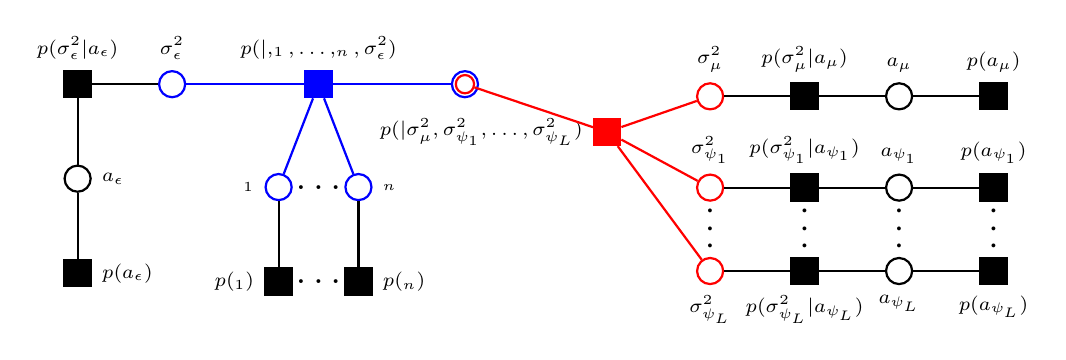
\begin{tikzpicture} [
		auto, node distance=1.2cm, every loop/.style={},
		thick,stochastic node/.style={circle,draw,font=\sffamily\Large\bfseries},
		factor/.style={regular polygon,regular polygon sides=4}
	]
	
	% Fragment for factor p(y | nu, zeta, sigsqeps):
	\node [
		fill = blue, factor, draw = blue, scale = 1,
		label = above:\scriptsize{$p ( \by | \bnu, \bzeta_1, \dots, \bzeta_n, \sigsqeps )$}
	] (py) {};
	\node [
		stochastic node, draw = blue, scale = 1,
		label = above:\scriptsize{$\bnu$}
	] (nu) [right = 1.5cm of py] {};
	\node [
		stochastic node, draw = blue, scale = 1,
		label = left:\scriptsize{$\bzeta_1$}
	] (zeta1) [below left = 1cm and 0.2cm of py] {};
	\node [
		stochastic node, draw = blue, scale=1,
		label = right:\scriptsize{$\bzeta_n$}
	] (zetaN) [below right = 1cm and 0.2cm of py] {};
	\node [font = \Large] (zeta_dots) at ($(zeta1)!0.54!(zetaN)$) {$\dots$};
	\node [
		stochastic node, draw = blue, scale=1,
		label = above:\scriptsize{$\sigsqeps$}
	] (sigsqeps) [left = 1.5cm of py] {};
	
	% Fragment for factor p(nu | sigsqmu, sigsqpsi1, ..., sigsqpsiL):
	\node [
		fill = red, factor, draw = red, scale = 1,
		label = left:\scriptsize{$p ( \bnu | \sigsqmu, \sigsqpsi{1}, \dots, \sigsqpsi{L} )$}
	] (pnu) [below right = 0.3cm and 1.5cm of nu] {};
	\node[stochastic node, draw = red, scale = 0.7] (nu_inner) at (nu.center) {};
	\node [
		stochastic node, draw = red, scale=1,
		label = above:\scriptsize{$\sigsqpsi{1}$}
	] (sigsqpsi1) [below right = 0.4cm and 1cm of pnu] {};
	\node [
		stochastic node, draw = red, scale=1,
		label = below:\scriptsize{$\sigsqpsi{L}$}
	] (sigsqpsiL) [below = 0.7cm of sigsqpsi1] {};
	\node [font = \Large, rotate=-90] (sigsqpsi_dots) at ($(sigsqpsi1)!0.53!(sigsqpsiL)$) {$\dots$};
	\node [
		stochastic node, draw = red, scale=1,
		label = above:\scriptsize{$\sigsqmu$}
	] (sigsqmu) [above = 0.8cm of sigsqpsi1] {};
	
	% Fragments for factors p(zeta1) ... p(zetaN):
	\node [
		fill, factor, draw, scale = 1,
		label = left:\scriptsize{$p ( \bzeta_1 )$}
	] (pzeta1) [below of =  zeta1] {};
	\node [
		fill, factor, draw, scale = 1,
		label = right:\scriptsize{$p ( \bzeta_n )$}
	] (pzetaN) [below of =  zetaN] {};
	\node [font = \Large] (pzeta_dots) at ($(pzeta1)!0.54!(pzetaN)$) {$\dots$};
	
	% Fragment for factor p(sigsqeps | aeps):
	\node [
		fill, factor, draw, scale = 1,
		label = above:\scriptsize{$p ( \sigsqeps | \aeps )$}
	] (psigsqeps) [left of = sigsqeps] {};
	\node [
		stochastic node, draw, scale=1,
		label = right:\scriptsize{$\aeps$}
	] (aeps) [below of = psigsqeps] {};
	
	% Fragment for factor p(aeps):
	\node [
		fill, factor, draw, scale = 1,
		label = right:\scriptsize{$p ( \aeps )$}
	] (paeps) [below of = aeps] {};
	
	% Fragment for factor p(sigsqmu | amu):
	\node [
		fill, factor, draw, scale = 1,
		label = above:\scriptsize{$p ( \sigsqmu | \amu )$}
	] (psigsqmu) [right of = sigsqmu] {};
	\node [
		stochastic node, draw, scale=1,
		label = above:\scriptsize{$\amu$}
	] (amu) [right of = psigsqmu] {};
	
	% Fragment for factor p(amu):
	\node [
		fill, factor, draw, scale = 1,
		label = above:\scriptsize{$p ( \amu )$}
	] (pamu) [right of = amu] {};
	
	% Fragments for factors p(sigsqpsi1 | apsi1) ... p(sigsqpsiL | apsiL):
	\node [
		fill, factor, draw, scale = 1,
		label = above:\scriptsize{$p ( \sigsqpsi{1} | \apsi{1} )$}
	] (psigsqpsi1) [right of = sigsqpsi1] {};
	\node [
		stochastic node, draw, scale = 1,
		label = above:\scriptsize{$ \apsi{1} $}
	] (apsi1) [right of = psigsqpsi1] {};
	\node [
		fill, factor, draw, scale = 1,
		label = below:\scriptsize{$p ( \sigsqpsi{L} | \apsi{L} )$}
	] (psigsqpsiL) [right of = sigsqpsiL] {};
	\node [
		stochastic node, draw, scale = 1,
		label = below:\scriptsize{$ \apsi{L} $}
	] (apsiL) [right of = psigsqpsiL] {};
	\node [font = \Large, rotate=-90] (psigsqpsi_dots) at ($(psigsqpsi1)!0.53!(psigsqpsiL)$) {$\dots$};
	\node [font = \Large, rotate=-90] (apsi_dots) at ($(apsi1)!0.53!(apsiL)$) {$\dots$};
	
	% Fragments for factors p(apsi1) ... p(apsiL):
	\node [
		fill, factor, draw, scale = 1,
		label = above:\scriptsize{$p ( \apsi{1} )$}
	] (papsi1) [right of = apsi1] {};
	\node [
		fill, factor, draw, scale = 1,
		label = below:\scriptsize{$p ( \apsi{L} )$}
	] (papsiL) [right of = apsiL] {};
	\node [font = \Large, rotate=-90] (papsi_dots) at ($(papsi1)!0.53!(papsiL)$) {$\dots$};
	
	% Construct edges:
	\path[every node/.style={font=\sffamily\small}]
	
	% Edges around fragment for factor p(y | nu, zeta1, ..., zetaN, sigsqeps):
	(py)
		edge [blue] node {} (nu)
		edge [blue] node {} (zeta1)
		edge [blue] node {} (zetaN)
		edge [blue] node {} (sigsqeps)
	
	% Edges around fragment for factor p(nu | sigsqmu, sigsqpsi1, ..., sigsqpsiL):
	(pnu)
		edge [red] node {} (nu_inner)
		edge [red] node {} (sigsqmu)
		edge [red] node {} (sigsqpsi1)
		edge [red] node {} (sigsqpsiL)
	
	% Edges around fragments for factors p(zeta1) ... p(zetaN):
	(pzeta1) edge node {} (zeta1)
	(pzetaN) edge node {} (zetaN)
	
	% Edges around fragment for factor p(sigsqeps | aeps):
	(psigsqeps)
		edge node {} (sigsqeps)
		edge node {} (aeps)
	
	% Edges around fragment for factor p(aeps):
	(paeps)
		edge node {} (aeps)
	
	% Edges around fragment for factor p(sigsqmu | amu):
	(psigsqmu)
		edge node {} (sigsqmu)
		edge node {} (amu)
	
	% Edges around fragment for factor p(amu):
	(pamu)
		edge node {} (amu)
	
	% Edges around fragments for factors p(sigsqpsi1 | apsi1) ... p(sigsqpsiL | apsiL):
	(psigsqpsi1)
		edge node {} (sigsqpsi1)
		edge node {} (apsi1)
	(psigsqpsiL)
		edge node {} (sigsqpsiL)
		edge node {} (apsiL)
	
	% Edges around fragments for factors p(apsi1) ... p(apsiL):
	(papsi1)
		edge node {} (apsi1)
	(papsiL)
		edge node {} (apsiL);
	
	\end{tikzpicture}
\caption{The factor graph for the Bayesian FPCA model in \eqref{bayes_fpca_mod}.}
\label{fig:fg_fpca}
\end{figure}

A key step in deriving and implementing VMP algorithms is the representation of probability density functions
in exponential family form: $p (\bx) \propto \exp \{ \T{\bT(x)} \bdeta \}$, where $\bT (x)$ is a vector of sufficient
statistics that identify the distributional family, and $\bdeta$ is the natural parameter vector;
the messages in \eqref{nu_zeta_q_dens_funcs} are typically in the exponential family of density functions.
\citet{wand17} explains how natural parameter vectors play a central role in the messages that are
passed within and between factor graph fragments. In particular, the natural parameter vectors for the
optimal $q$-density functions in \eqref{nu_zeta_q_dens_funcs} take the form

\begin{align}
\begin{split}
	\npq{\bnu} &=
		\np{p (\by | \bnu, \bzeta_1, \dots, \bzeta_n, \sigsqeps)}{\bnu} +
		\np{p (\bnu | \sigsqmu, \sigsqpsi{1}, \dots, \sigsqpsi{L})}{\bnu} \\
	\npq{\bzeta_i} &=
		\np{p (\by | \bnu, \bzeta_1, \dots, \bzeta_n, \sigsqeps)}{\bzeta_i} +
		\np{p (\bzeta_i)}{\bzeta_i} , \quad i = 1, \dots, n.
\end{split}
\label{etaq}
\end{align}

\noindent We outline the exponential family form of the normal and inverse-$\chi^2$ density functions in
Appendix \ref{app:exp_fam_form}.

We introduce two new fragments that are required for variational inference via VMP for the FPCA model. These
are the \emph{functional principal component Gaussian likelihood fragment} (blue in Figure \ref{fig:fg_fpca})
and the \emph{multiple Gaussian penalization fragment} (red in Figure \ref{fig:fg_fpca}).
The fragments for $p (\bzeta_1), \dots, p (\bzeta_n)$ are \emph{Gaussian prior fragments}
\cite[Section~4.1.1]{wand17}; the fragments for $p (\sigsqeps | \aeps)$, $p (\sigsqmu | \amu)$ and
$p (\sigsqpsi{1} | \apsi{1}), \dots, p (\sigsqpsi{L} | \apsi{L})$ are univariate versions of the \emph{iterated inverse
G-Wishart fragment} \cite[Algorithm~2]{maestrini20}; and $p (\aeps)$, $p (\amu)$ and $p (\apsi{1}), \dots, p (\apsi{L})$
are univariate versions of the \emph{inverse G-Wishart prior fragment} \cite[Algorithm~1]{maestrini20}.

%%%%%%%%%%%%%% Functional Principal Component Gaussian Likelihood Fragment

\subsection{Functional Principal Component Gaussian Likelihood Fragment}
\label{sec:fpca_gauss_lik_frag}

The message from $p (\by | \bnu, \bzeta_1, \dots, \bzeta_n, \sigsqeps)$ to $\bnu$ can be shown to be
proportional to a multivariate normal density function, with natural parameter vector

\begin{equation}
	\np{p (\by | \bnu, \bzeta_1, \dots, \bzeta_n, \sigsqeps)}{\bnu}
		\longleftarrow
			\begin{bmatrix}
				\E_q (1/\sigsqeps) \displaystyle\sum_{i=1}^n \T{\left\{
					\T{\E_q (\bzetatilde_i)} \otimes \bC_i
				\right\}} \by_i \\
				-\frac12 \E_q (1/\sigsqeps) \displaystyle\sum_{i=1}^n \vect \left\{
					\E_q (\bzetatilde_i \T{\bzetatilde_i}) \otimes (\T{\bC_i} \bC_i)
				\right\}
			\end{bmatrix},
\label{np_lik_nu}
\end{equation}

\noindent where $\bzetatilde_i \equiv \T{(1, \T{\bzeta_i})}, \ i = 1, \dots, n$.

%Note that the natural
%parameter vector in \eqref{np_lik_nu} is within the vec-based representation of a normal probability density function.
%In preliminary simulations, we found that computations using the vech-based representation were enormously hindered
%by the need to use a huge Moore-Penrose inverse matrix. For instance, consider the case where
%there are two basis functions ($L = 2$) and 25 O'Sullivan penalized spline basis functions ($K = 25$) for nonparametric
%regression. In this instance, the vector $\bnu$ is $81 \times 1$ ($d = 81$) and the Moore-Penrose inverse matrix
%$\bD_{81}^+$ has dimension $3321 \times 6561$, inhibiting the computational speed. For this reason, we have
%decided to use the vec-based representation for $\msg{p (\by | \bnu, \bzeta_1, \dots, \bzeta_n, \sigsqeps)}{\bnu}$,
%which does not require the
%use of a Moore-Penrose inverse matrix.

For each $i = 1, \dots, n$, the message from $p (\by | \bnu, \bzeta_1, \dots, \bzeta_n, \sigsqeps)$ to $\bzeta_i$
is proportional to a multivariate normal density function, with natural parameter vector

\begin{equation}
	\np{p (\by | \bnu, \bzeta_1, \dots, \bzeta_n, \sigsqeps)}{\bzeta_i}
		\longleftarrow
			\begin{bmatrix}
				\E_q (1/\sigsqeps) \left\{
					\T{\E_q (\Vpsi)} \T{\bC_i} \by_i - \E_q (\hmupsi{i})
				\right\} \\
				-\frac12 \E_q (1/\sigsqeps) \T{\bD_L} \vect \{ \E_q (\Hpsi{i}) \}
			\end{bmatrix},
\label{np_lik_zeta}
\end{equation}

\noindent where $ \Vpsi \equiv [\begin{array}{ccc} \nupsi{1} & \dots & \nupsi{L} \end{array}]$,
$\hmupsi{i} \equiv \T{\Vpsi} \T{\bC_i} \bC_i \numu$ and $\Hpsi{i} \equiv \T{\Vpsi} \T{\bC_i} \bC_i \Vpsi$.

The message from $p (\by | \bnu, \bzeta_1, \dots, \bzeta_n, \sigsqeps)$ to $\sigsqeps$
is an inverse-$\chi^2$ density function, with natural parameter vector

\begin{equation}
	\np{p (\by | \bnu, \bzeta_1, \dots, \bzeta_n, \sigsqeps)}{\sigsqeps}
		\longleftarrow
			\begin{bmatrix}
				-\frac12 \displaystyle\sum_{i=1}^n T_i \\
				-\frac12 \displaystyle\sum_{i=1}^n \E_q \left\{ \T{\left(
					\by_i - \bC_i \bV \bzetatilde_i
				\right)} \left(
					\by_i - \bC_i \bV \bzetatilde_i
				\right) \right\}
			\end{bmatrix},
\label{np_lik_sigsqeps}
\end{equation}

\noindent where $\bV \equiv [\begin{array}{cccc} \numu & \nupsi{1} & \dots & \nupsi{L} \end{array}]$.

%Note that the inverse-$\chi^2$ density function message that is passed
%to $\sigsqeps$ is part of the inverse G-Wishart class of density functions. In keeping
%with the formalisms set out in \citet{maestrini20},
%a graph message is also required for conjugate variational inference.
%According to Section 7.4 of \citet{maestrini20},
%the auxiliary-based hierarchical prior specification of $\sigsqeps$ in \eqref{bayes_fpca_mod} requires a
%graphical message of the form

%\begin{equation}
%	G_{p (\by | \bnu, \bzeta_1, \dots, \bzeta_n, \sigsqeps) \rightarrow \sigsqeps}
%		\longleftarrow
%			G_{\text{full}}.
%\label{G_lik_sigsqeps}
%\end{equation}

%\noindent See \citet{maestrini20} for further details on graphical parameters in inverse G-Wishart and\
%inverse-$\chi^2$ density functions.

Pseudocode for the functional principal component
Gaussian likelihood fragment is presented in Algorithm \ref{alg:fpca_gauss_lik_frag}.
A derivation of all the relevant expectations and natural parameter vector updates is provided in Appendix
\ref{app:fpca_gauss_lik_frag}.

\begin{algorithm}
	\caption{
		Pseudocode for the functional principal component Gaussian likelihood fragment.
	}
	\label{alg:fpca_gauss_lik_frag}
	\begin{algorithmic}[1]
		\Inputs $
				\npq{\bnu}, \quad
				\{ \npq{\bzeta_i} : i = 1, \dots, n \}, \quad
				\npq{\sigsqeps}
		$
		\Updates
			\State Update posterior expectations.
				\Comment{see Appendix \ref{app:fpca_gauss_lik_frag}}
			\State Update $\np{p (\by | \bnu, \bzeta_1, \dots, \bzeta_n, \sigsqeps)}{\bnu}$
				\Comment{equation \eqref{np_lik_nu}}
			\For{$i = 1, \dots, n$}
				\State Update $\np{p (\by | \bnu, \bzeta_1, \dots, \bzeta_n, \sigsqeps)}{\bzeta_i}$
					\Comment{equation \eqref{np_lik_zeta}}
			\EndFor
			\State Update $\np{p (\by | \bnu, \bzeta_1, \dots, \bzeta_n, \sigsqeps)}{\sigsqeps}$
				\Comment{equation \eqref{np_lik_sigsqeps}}
%			\State Update $G_{p (\by | \bnu, \bzeta_1, \dots, \bzeta_n, \sigsqeps) \rightarrow \sigsqeps}$
%				\Comment{equation \eqref{G_lik_sigsqeps}}
		\Outputs
			\begin{varwidth}[t]{\linewidth} $
				\np{p (\by | \bnu, \bzeta_1, \dots, \bzeta_n, \sigsqeps)}{\bnu}, \quad
				\{ \np{p (\by | \bnu, \bzeta_1, \dots, \bzeta_n, \sigsqeps)}{\bzeta_i} : i = 1, \dots, n \}
			$\par$
%				\{
					\np{p (\by | \bnu, \bzeta_1, \dots, \bzeta_n, \sigsqeps)}{\sigsqeps}
%					G_{p (\by | \bnu, \bzeta_1, \dots, \bzeta_n, \sigsqeps) \rightarrow \sigsqeps}
%				\}
			$ \end{varwidth}
	\end{algorithmic}
\end{algorithm}

%%%%%%%%%%%%%% Multiple Gaussian Penalization Fragment

\subsection{Multiple Gaussian Penalization Fragment}
\label{sec:mean_fpc_gauss_pen_frag}

The message passed from $p (\bnu | \sigsqmu, \sigsqpsi{1}, \dots, \sigsqpsi{L})$ to $\bnu$ can be shown to
be a multivariate normal density function, with natural parameter vector

\begin{equation}
	\np{p (\bnu | \sigsqmu, \sigsqpsi{1}, \dots, \sigsqpsi{L})}{\bnu}
		\longleftarrow
			\begin{bmatrix}
				\bzero_{d} \\
				-\frac12 \vect \left\{ \E_q (\Sigmanu^{-1}) \right\}
			\end{bmatrix},
\label{np_pen_nu}
\end{equation}

\noindent where $\Sigmanu \equiv \blockdiag (\bSigma_\mu, \bSigma_{\psi_1}, \dots, \bSigma_{\psi_L})$.
%The natural parameter vector in \eqref{np_pen_nu} is within the
%vec-based representation of the message to $\bnu$, as opposed to
%a storage-economical vech-based representation, for the same reasons that are outlined in the discussion
%following \eqref{np_lik_nu}.

The message from $p (\bnu | \sigsqmu, \sigsqpsi{1}, \dots, \sigsqpsi{L})$ to $\sigsqmu$ is an inverse-$\chi^2$
density function, with natural parameter vector

\begin{equation}
	\np{p (\bnu | \sigsqmu, \sigsqpsi{1}, \dots, \sigsqpsi{L})}{\sigsqmu}
		\longleftarrow
			\begin{bmatrix}
				-\frac{K}{2} \\
				-\frac12 \E_q (\T{\umu} \umu)
			\end{bmatrix}.
\label{np_pen_sigsqmu}
\end{equation}

Similarly, the message passed from $p (\bnu | \sigsqmu, \sigsqpsi{1}, \dots, \sigsqpsi{L})$ to $\sigsqpsi{l}$,
$l = 1, \dots, L$, is an inverse-$\chi^2$ density function, with natural parameter vector

\begin{equation}
	\np{p (\bnu | \sigsqmu, \sigsqpsi{1}, \dots, \sigsqpsi{L})}{\sigsqpsi{l}}
		\longleftarrow
			\begin{bmatrix}
				-\frac{K}{2} \\
				-\frac12 \E_q (\T{\upsi{l}} \upsi{l})
			\end{bmatrix}.
\label{np_pen_sigsqpsi}
\end{equation}

%Finally, recall the discussion following \eqref{np_lik_sigsqeps}.
%Each of the messages to the variance parameters $\sigsqmu,
%\sigsqpsi{1}, \dots, \sigsqpsi{L}$ must be paired with a graph message. For the same reasons that were used to
%justify the graphical message in \eqref{G_lik_sigsqeps}, the graph messages received by $\sigsqmu,
%\sigsqpsi{1}, \dots, \sigsqpsi{L}$ are, respectively,

%\begin{equation}
%	G_{p (\bnu | \sigsqmu, \sigsqpsi{1}, \dots, \sigsqpsi{L}) \rightarrow \sigsqmu}
%		\longleftarrow
%			G_{\text{full}} \quad
%	\text{and} \quad
%	G_{p (\bnu | \sigsqmu, \sigsqpsi{1}, \dots, \sigsqpsi{L}) \rightarrow \sigsqpsi{l}}
%		\longleftarrow
%			G_{\text{full}}, \quad l = 1, \dots, L.
%\label{G_pen}
%\end{equation}

Pseudocode for the multiple Gaussian penalization fragment is presented in Algorithm
\ref{alg:mean_fpc_gauss_pen_frag}.
A derivation of all the relevant expectations and natural parameter vector updates is provided in Appendix
\ref{app:mean_fpc_gauss_pen_frag}.

\begin{algorithm}
	\caption{
		Pseudocode for the multiple Gaussian penalization fragment.
	}
	\label{alg:mean_fpc_gauss_pen_frag}
	\begin{algorithmic}[1]
		\Inputs $
				\npq{\bnu}, \quad
				\npq{\sigsqmu}, \quad
				\{
					\npq{\sigsqpsi{l}}:
					l = 1, \dots, L
				\}
		$
		\Updates
			\State Update posterior expectations.
				\Comment{see Appendix \ref{app:mean_fpc_gauss_pen_frag}}
			\State Update $\np{p (\bnu | \sigsqmu, \sigsqpsi{1}, \dots, \sigsqpsi{L})}{\bnu}$
				\Comment{equation \eqref{np_pen_nu}}
			\State Update $\np{p (\bnu | \sigsqmu, \sigsqpsi{1}, \dots, \sigsqpsi{L})}{\sigsqmu}$
				\Comment{equation \eqref{np_pen_sigsqmu}}
%			\State Update $G_{p (\bnu | \sigsqmu, \sigsqpsi{1}, \dots, \sigsqpsi{L}) \rightarrow \sigsqmu}$
%				\Comment{equation \eqref{G_pen}}
			\For{$l = 1, \dots, L$}
				\State Update $\np{p (\bnu | \sigsqmu, \sigsqpsi{1}, \dots, \sigsqpsi{L})}{\sigsqpsi{l}}$
					\Comment{equation \eqref{np_pen_sigsqpsi}}
%				\State Update $G_{p (\bnu | \sigsqmu, \sigsqpsi{1}, \dots, \sigsqpsi{L}) \rightarrow \sigsqpsi{l}}$
%					\Comment{equation \eqref{G_pen}}
			\EndFor
		\Outputs
			\begin{varwidth}[t]{\linewidth} $
				\np{p (\bnu | \sigsqmu, \sigsqpsi{1}, \dots, \sigsqpsi{L})}{\bnu}, \quad
%				\{
					\np{p (\bnu | \sigsqmu, \sigsqpsi{1}, \dots, \sigsqpsi{L})}{\sigsqmu},
%					G_{p (\bnu | \sigsqmu, \sigsqpsi{1}, \dots, \sigsqpsi{L}) \rightarrow \sigsqmu}
%				\}
			$\par$
				\{
					\np{p (\bnu | \sigsqmu, \sigsqpsi{1}, \dots, \sigsqpsi{L})}{\sigsqpsi{l}} :
%					G_{p (\bnu | \sigsqmu, \sigsqpsi{1}, \dots, \sigsqpsi{L}) \rightarrow \sigsqpsi{l}} :
					l = 1, \dots, L
				\}
			$ \end{varwidth}
	\end{algorithmic}
\end{algorithm}

Note that the multiple Gaussian penalization fragment is not a fragment designed specifically for
orthogonal FPCA because it
does not account for an orthogonal set of basis functions. Indeed, it can be applied to any statistical
model that specifies an independent penalization structure over mulitple vectors of spline coefficients.

%%%%%%%%%%%%%%  MULTILEVEL  EXTENSIONS  %%%%%%%%%%%%%%%

\section{Multilevel Extensions}
\label{sec:mlfpca}

\citet{di09} introduces multilevel FPCA (MlFPCA) for clustered or multilevel functional data. The multilevel
extension of \eqref{yhat}, which is a simplified version the MlFPCA model in \citet{di09}, is

\begin{equation}
	\yhat_{ij} (t) =
		\mu (t) + \sum_{l = 1}^{L_1} \zetaL{1}{il} \psiL{1}{l} (t)
		+ \sum_{l = 1}^{L_2} \zetaL{2}{ijl} \psiL{2}{l} (t),
	\quad j = 1, \dots, m_i, \quad i = 1, \dots, n.
\label{yhatml}
\end{equation}

\noindent The first level eigenfunctions $\{ \psiL{1}{l} \}_{l = 1, \dots, L_1}$ account for first level specific
shifts from the mean function $\mu (t)$, and the second level eigenfunctions $\{ \psiL{2}{l} \}_{l = 1, \dots, L_2}$
account for second level specific shifts from the subject-specific mean function.
Note that the level one and level two eigenfunctions form an orthonormal
basis, but are not required to be mutually orthogonal. With the assumption of Gaussian residuals, the first level
scores $\zetaL{1}{il}$ are uncorrelated zero-mean Gaussian random variables, and likewise for the second
level scores $\zetaL{2}{ijl}$. Additionally, first and second level scores are assumed to be uncorrelated.
A similar MlFPCA decomposition was used in \citet{Goldsmith15} for generalized multilevel
function-on-scalar regression.

In constructing the Bayesian model, we note that the multivariate extension of \eqref{resp_mod} is

\[
	\by_{ij} =
		\bmu_{ij} + \sum_{l=1}^{L_1} \zetaL{1}{il} \bpsiL{1}{ijl}
		+ \sum_{l=1}^{L_2} \zetaL{2}{ijl} \bpsiL{2}{ijl} + \bepsilon_{ij},
	\quad j = 1, \dots, m_i, \quad i = 1, \dots, n,
\]

\noindent where $\by_{ij}, \bmu_{ij}, \{ \bpsiL{1}{ijl} \}_{l = 1, \dots, L_1}$ and $\{ \bpsiL{2}{ijl} \}_{l = 1, \dots, L_2}$
are $T_{ij} \times 1$ vectors defined over the design points $t_{ij1}, \dots, t_{ijT_{ij}}$ for the $ij$th observation.
For nonparametric fitting of the nonlinear curves in the model, the design matrix $\bC_{ij}$ has an identical
structure to \eqref{C_mat}, but evaluated of the design points $t_{ij1}, \dots, t_{ijT_{ij}}$. Vectors of spline
coefficients are defined as $\numu, \{ \nupsiL{1}{l} \}_{l = 1, \dots, L_1}$ and $\{ \nupsiL{2}{l} \}_{l = 1, \dots, L_2}$
for the mean function, the first level eigenfunctions, and the second level eigenfunctions, respectively.
Vectors of scores are defined such that $\bzetaL{1}{i} \equiv \T{(\zetaL{1}{i1}, \dots, \zetaL{1}{iL_1})}$ and
$\bzetaL{2}{ij} \equiv \T{(\zetaL{2}{ij1}, \dots, \zetaL{1}{ijL_2})}$. In addition, we will introduce a slight abuse
of notation by setting $L \equiv L_1 + L_2$,
$\bnu \equiv \T{(\T{\numu}, \nupsiTL{1}{1}, \dots, \nupsiTL{1}{L_1}, \nupsiTL{2}{1}, \dots, \nupsiTL{2}{L_2})}$
and $\bzeta_i \equiv \T{(\bzetaTL{1}{i}, \bzetaTL{2}{i1}, \dots, \bzetaTL{2}{im_i})}$ for $i = 1, \dots, n$
in the multilevel setting. However, the precise definition of $L$, $\bnu$ and $\bzeta_i$ should be apparent from
the specific model (standard or multilevel) that we are analysing.


The Bayesian MlFPCA model is:

\begin{equation}
\begin{gathered}
	\by_{ij} | \bnu, \bzetaL{1}{i}, \bzetaL{2}{ij}, \sigsqeps \indsim \normal \left\{
		\bC_{ij} \left(
			\numu + \sum_{l=1}^{L_1} \zetaL{1}{il} \nupsiL{1}{l}
			+ \sum_{l=1}^{L_2} \zetaL{2}{ijl} \nupsiL{2}{l}
		\right),
		\sigsqeps \bI_{T_{ij}}
	\right\}, \\
	$$
	\bzetaL{1}{i} \indsim \normal (\bzero, \bI), \quad
	\bzetaL{2}{ij} \indsim \normal (\bzero, \bI), \quad
	j = 1, \dots, m_i, \quad i = 1, \dots, n, \\
	$$
	\left.\begin{bmatrix}
		\numu \\
		\nupsiL{1}{l} \\
		\nupsiL{2}{k}
	\end{bmatrix} \ \right| \ \sigsqmu, \sigsqpsiL{1}{l}, \sigsqpsiL{2}{k}
		\indsim
			\normal \left(
				\begin{bmatrix}
					\bzero \\
					\bzero \\
					\bzero
				\end{bmatrix},
				\begin{bmatrix}
					\bSigma_\mu & \textbf{O} & \textbf{O} \\
					\textbf{O} & \bSigma^{(1)}_{\psi_l} & \textbf{O} \\
					\textbf{O} & \textbf{O} & \bSigma^{(2)}_{\psi_k}
				\end{bmatrix}
			\right), \\
	$$
	\sigsqpsiL{1}{l} | \apsiL{1}{l} \indsim \invchisq (1, 1/\apsiL{1}{l}), \quad
	\apsiL{1}{l} \indsim \invchisq (1, 1/A^2), \quad l = 1, \dots, L_1, \\
	$$
	\sigsqpsiL{2}{k} | \apsiL{2}{k} \indsim \invchisq (1, 1/\apsiL{2}{k}), \quad
	\apsiL{2}{k} \indsim \invchisq (1, 1/A^2), \quad k = 1, \dots, L_2, \\
	$$
	\sigsqmu | \amu \sim \invchisq (1, 1/\amu), \quad \amu \sim \invchisq(1, 1/A^2), \\
	$$
	\sigsqeps | \aeps \sim \invchisq (1, 1/\aeps), \quad \aeps \sim \invchisq(1, 1/A^2).
\end{gathered}
\label{bayes_mlfpca_mod}
\end{equation}

%%%%%%%%%%%%%% VMP for MlFPCA

\subsection{VMP for MlFPCA}
\label{sec:vmp_mlfpca}

The mean field restriction that we set for model \eqref{bayes_mlfpca_mod}, after applying induced
factorizations similar to those used to derive \eqref{fpca_mf_restrn}, is:

\begin{align}
\begin{split}
	q (
		\bnu, &\{ \bzeta_i \}_{i = 1, \dots, n},
		\sigsqeps, \aeps, \sigsqmu, \amu,
		\{ \sigsqpsiL{1}{l}, \apsiL{1}{l} \}_{l = 1, \dots, L_1},
		\{ \sigsqpsiL{2}{l}, \apsiL{2}{l} \}_{l = 1, \dots, L_2}) \\
		=
			&\left\{ \prod_{i=1}^n q (\bzeta_i) \right\}
			q (\bnu) q(\sigsqeps) q(\aeps) q(\sigsqmu) q (\amu)
			\left\{ \prod_{l=1}^{L_1} q(\sigsqpsiL{1}{l}) q(\apsiL{1}{l}) \right\}
			\left\{ \prod_{l=1}^{L_2} q(\sigsqpsiL{2}{l}) q(\apsiL{2}{l}) \right\}.
\end{split}
\label{mlfpca_mf_restrn}
\end{align}

\noindent The factor graph for model \eqref{bayes_mlfpca_mod} that represents the factorization in
\eqref{mlfpca_mf_restrn} is presented in Figure \ref{fig:fg_mlfpca}.

\begin{figure}
	\centering
	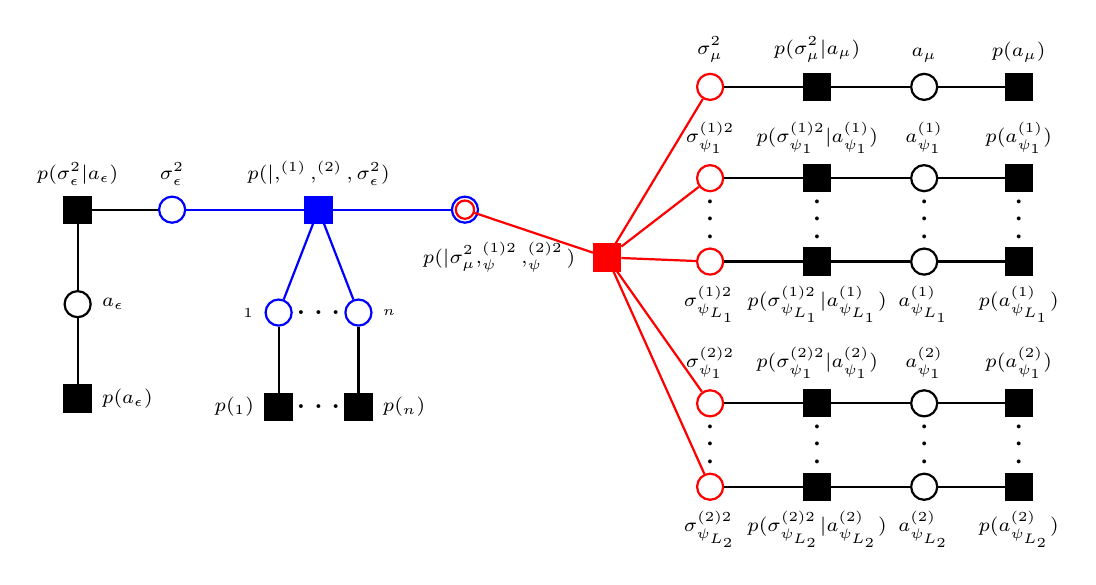
\begin{tikzpicture} [
		auto, node distance=1.2cm, every loop/.style={},
		thick,stochastic node/.style={circle,draw,font=\sffamily\Large\bfseries},
		factor/.style={regular polygon,regular polygon sides=4}
	]
	
	% Fragment for factor p(y | nu, zeta^1, zeta^2, sigsqeps):
	\node [
		fill = blue, factor, draw = blue, scale = 1,
		label = above:\scriptsize{$p ( \by | \bnu, \bzetaL{1}{}, \bzetaL{2}{}, \sigsqeps )$}
	] (py) {};
	\node [
		stochastic node, draw = blue, scale = 1,
		label = above:\scriptsize{$\bnu$}
	] (nu) [right = 1.5cm of py] {};
	\node [
		stochastic node, draw = blue, scale = 1,
		label = left:\scriptsize{$\bzeta_1$}
	] (zeta1) [below left = 1cm and 0.2cm of py] {};
	\node [
		stochastic node, draw = blue, scale=1,
		label = right:\scriptsize{$\bzeta_n$}
	] (zetaN) [below right = 1cm and 0.2cm of py] {};
	\node [font = \Large] (zeta_dots) at ($(zeta1)!0.54!(zetaN)$) {$\dots$};
	\node [
		stochastic node, draw = blue, scale=1,
		label = above:\scriptsize{$\sigsqeps$}
	] (sigsqeps) [left = 1.5cm of py] {};
	
	% Fragment for factor p(nu | sigsqmu, sigsqpsi11, ..., sigsqpsi1L):
	\node [
		fill = red, factor, draw = red, scale = 1,
		label = left:\scriptsize{$p ( \bnu | \sigsqmu, \bsigma^{(1) 2}_\psi, \bsigma^{(2) 2}_\psi ) \ $}
	] (pnu) [below right = 0.3cm and 1.5cm of nu] {};
	\node[stochastic node, draw = red, scale = 0.7] (nu_inner) at (nu.center) {};
	\node [
		stochastic node, draw = red, scale=1,
		label = above:\scriptsize{$\sigsqpsiL{1}{1}$}
	] (sigsqpsi11) [above right = 0.7cm and 1cm of pnu] {};
	\node [
		stochastic node, draw = red, scale=1,
		label = below:\scriptsize{$\sigsqpsiL{1}{L_1}$}
	] (sigsqpsi1L) [below = 0.7cm of sigsqpsi11] {};
	\node [font = \Large, rotate=-90] (sigsqpsi1_dots) at ($(sigsqpsi11)!0.53!(sigsqpsi1L)$) {$\dots$};
	\node [
		stochastic node, draw = red, scale=1,
		label = above:\scriptsize{$\sigsqmu$}
	] (sigsqmu) [above = 0.8cm of sigsqpsi11] {};
	\node [
		stochastic node, draw = red, scale=1,
		label = above:\scriptsize{$\sigsqpsiL{2}{1}$}
	] (sigsqpsi21) [below = 2.5cm of sigsqpsi11] {};
	\node [
		stochastic node, draw = red, scale=1,
		label = below:\scriptsize{$\sigsqpsiL{2}{L_2}$}
	] (sigsqpsi2L) [below = 0.7cm of sigsqpsi21] {};
	\node [font = \Large, rotate=-90] (sigsqpsi2_dots) at ($(sigsqpsi21)!0.53!(sigsqpsi2L)$) {$\dots$};
	
	% Fragments for factors p(zeta1) ... p(zetaN):
	\node [
		fill, factor, draw, scale = 1,
		label = left:\scriptsize{$p ( \bzeta_1 )$}
	] (pzeta1) [below of =  zeta1] {};
	\node [
		fill, factor, draw, scale = 1,
		label = right:\scriptsize{$p ( \bzeta_n )$}
	] (pzetaN) [below of =  zetaN] {};
	\node [font = \Large] (pzeta_dots) at ($(pzeta1)!0.54!(pzetaN)$) {$\dots$};
	
	% Fragment for factor p(sigsqeps | aeps):
	\node [
		fill, factor, draw, scale = 1,
		label = above:\scriptsize{$p ( \sigsqeps | \aeps )$}
	] (psigsqeps) [left of = sigsqeps] {};
	\node [
		stochastic node, draw, scale=1,
		label = right:\scriptsize{$\aeps$}
	] (aeps) [below of = psigsqeps] {};
	
	% Fragment for factor p(aeps):
	\node [
		fill, factor, draw, scale = 1,
		label = right:\scriptsize{$p ( \aeps )$}
	] (paeps) [below of = aeps] {};
	
	% Fragment for factor p(sigsqmu | amu):
	\node [
		fill, factor, draw, scale = 1,
		label = above:\scriptsize{$p ( \sigsqmu | \amu )$}
	] (psigsqmu) [right = 1cm of sigsqmu] {};
	\node [
		stochastic node, draw, scale=1,
		label = above:\scriptsize{$\amu$}
	] (amu) [right = 1cm of psigsqmu] {};
	
	% Fragment for factor p(amu):
	\node [
		fill, factor, draw, scale = 1,
		label = above:\scriptsize{$p ( \amu )$}
	] (pamu) [right of = amu] {};
	
	% Fragments for factors p(sigsqpsi11 | apsi11) ... p(sigsqpsi1L | apsi1L):
	\node [
		fill, factor, draw, scale = 1,
		label = above:\scriptsize{$p ( \sigsqpsiL{1}{1} | \apsiL{1}{1} )$}
	] (psigsqpsi11) [right = 1cm of sigsqpsi11] {};
	\node [
		stochastic node, draw, scale = 1,
		label = above:\scriptsize{$ \apsiL{1}{1} $}
	] (apsi11) [right = 1cm of psigsqpsi11] {};
	\node [
		fill, factor, draw, scale = 1,
		label = below:\scriptsize{$p ( \sigsqpsiL{1}{L_1} | \apsiL{1}{L_1} )$}
	] (psigsqpsi1L) [right = 1cm of sigsqpsi1L] {};
	\node [
		stochastic node, draw, scale = 1,
		label = below:\scriptsize{$ \apsiL{1}{L_1} $}
	] (apsi1L) [right = 1cm of psigsqpsi1L] {};
	\node [font = \Large, rotate=-90] (psigsqpsi1_dots) at ($(psigsqpsi11)!0.53!(psigsqpsi1L)$) {$\dots$};
	\node [font = \Large, rotate=-90] (apsi1_dots) at ($(apsi11)!0.53!(apsi1L)$) {$\dots$};
	
	% Fragments for factors p(sigsqpsi21 | apsi21) ... p(sigsqpsi2L | apsi2L):
	\node [
		fill, factor, draw, scale = 1,
		label = above:\scriptsize{$p ( \sigsqpsiL{2}{1} | \apsiL{2}{1} )$}
	] (psigsqpsi21) [right = 1cm of sigsqpsi21] {};
	\node [
		stochastic node, draw, scale = 1,
		label = above:\scriptsize{$ \apsiL{2}{1} $}
	] (apsi21) [right = 1cm of psigsqpsi21] {};
	\node [
		fill, factor, draw, scale = 1,
		label = below:\scriptsize{$p ( \sigsqpsiL{2}{L_2} | \apsiL{2}{L_2} )$}
	] (psigsqpsi2L) [right = 1cm of sigsqpsi2L] {};
	\node [
		stochastic node, draw, scale = 1,
		label = below:\scriptsize{$ \apsiL{2}{L_2} $}
	] (apsi2L) [right = 1cm of psigsqpsi2L] {};
	\node [font = \Large, rotate=-90] (psigsqpsi2_dots) at ($(psigsqpsi21)!0.53!(psigsqpsi2L)$) {$\dots$};
	\node [font = \Large, rotate=-90] (apsi2_dots) at ($(apsi21)!0.53!(apsi2L)$) {$\dots$};
	
	% Fragments for factors p(apsi11) ... p(apsi1L):
	\node [
		fill, factor, draw, scale = 1,
		label = above:\scriptsize{$p ( \apsiL{1}{1} )$}
	] (papsi11) [right of = apsi11] {};
	\node [
		fill, factor, draw, scale = 1,
		label = below:\scriptsize{$p ( \apsiL{1}{L_1} )$}
	] (papsi1L) [right of = apsi1L] {};
	\node [font = \Large, rotate=-90] (papsi1_dots) at ($(papsi11)!0.53!(papsi1L)$) {$\dots$};
	
	% Fragments for factors p(apsi21) ... p(apsi2L):
	\node [
		fill, factor, draw, scale = 1,
		label = above:\scriptsize{$p ( \apsiL{2}{1} )$}
	] (papsi21) [right of = apsi21] {};
	\node [
		fill, factor, draw, scale = 1,
		label = below:\scriptsize{$p ( \apsiL{2}{L_2} )$}
	] (papsi2L) [right of = apsi2L] {};
	\node [font = \Large, rotate=-90] (papsi2_dots) at ($(papsi21)!0.53!(papsi2L)$) {$\dots$};
	
	% Construct edges:
	\path[every node/.style={font=\sffamily\small}]
	
	% Edges around fragment for factor p(y | nu, zeta1, ..., zetaN, sigsqeps):
	(py)
		edge [blue] node {} (nu)
		edge [blue] node {} (zeta1)
		edge [blue] node {} (zetaN)
		edge [blue] node {} (sigsqeps)
	
	% Edges around fragment for factor p(nu | sigsqmu, sigsqpsi11, ..., sigsqpsi1L):
	(pnu)
		edge [red] node {} (nu_inner)
		edge [red] node {} (sigsqmu)
		edge [red] node {} (sigsqpsi11)
		edge [red] node {} (sigsqpsi1L)
		edge [red] node {} (sigsqpsi21)
		edge [red] node {} (sigsqpsi2L)
	
	% Edges around fragments for factors p(zeta1) ... p(zetaN):
	(pzeta1) edge node {} (zeta1)
	(pzetaN) edge node {} (zetaN)
	
	% Edges around fragment for factor p(sigsqeps | aeps):
	(psigsqeps)
		edge node {} (sigsqeps)
		edge node {} (aeps)
	
	% Edges around fragment for factor p(aeps):
	(paeps)
		edge node {} (aeps)
	
	% Edges around fragment for factor p(sigsqmu | amu):
	(psigsqmu)
		edge node {} (sigsqmu)
		edge node {} (amu)
	
	% Edges around fragment for factor p(amu):
	(pamu)
		edge node {} (amu)
	
	% Edges around fragments for factors p(sigsqpsi11 | apsi11) ... p(sigsqpsi1L | apsi1L):
	(psigsqpsi11)
		edge node {} (sigsqpsi11)
		edge node {} (apsi11)
	(psigsqpsi1L)
		edge node {} (sigsqpsi1L)
		edge node {} (apsi1L)
	
	% Edges around fragments for factors p(sigsqpsi21 | apsi21) ... p(sigsqpsi2L | apsi2L):
	(psigsqpsi21)
		edge node {} (sigsqpsi21)
		edge node {} (apsi21)
	(psigsqpsi2L)
		edge node {} (sigsqpsi2L)
		edge node {} (apsi2L)
	
	% Edges around fragments for factors p(apsi11) ... p(apsi1L):
	(papsi11)
		edge node {} (apsi11)
	(papsi1L)
		edge node {} (apsi1L)
	
	% Edges around fragments for factors p(apsi21) ... p(apsi2L):
	(papsi21)
		edge node {} (apsi21)
	(papsi2L)
		edge node {} (apsi2L);
	
	\end{tikzpicture}
\caption{
	The factor graph for the Bayesian MlFPCA model in \eqref{bayes_mlfpca_mod}. To avoid notational
	clutter within the factor graph, we have introduced some notation: we set
	$\bsigma^{(1) 2}_\psi = \{ \sigsqpsiL{1}{l} \}_{l = 1, \dots, L_1}$ and
	$\bsigma^{(1) 2}_\psi = \{ \sigsqpsiL{2}{l} \}_{l = 1, \dots, L_2}$.
}
\label{fig:fg_mlfpca}
\end{figure}

In extending the Bayesian FPCA model to its multilevel form, we can see the advantage of using a VMP
approach to variational Bayesian inference. First note the fragments that have been derived
in previous publications:
the fragments for $p (\sigsqeps | \aeps)$, $p (\sigsqpsiL{1}{1} | \apsiL{1}{1}), \dots,
p (\sigsqpsiL{1}{L_1} | \apsiL{1}{L_1})$ and $p (\sigsqpsiL{2}{1} | \apsiL{2}{1}), \dots,
p (\sigsqpsiL{2}{L_2} | \apsiL{2}{L_2})$ are univariate versions of the iterated inverse G-Wishart fragment;
and the fragments for
$p (\aeps)$, $p (\apsiL{1}{1}), \allowbreak \dots, p (\apsiL{1}{L_1})$ and $p (\apsiL{1}{1}), \dots,
p (\apsiL{1}{L_1})$ are univariate versions of the inverse G-Wishart prior fragment. Next, we focus on
the fragment colored in red in Figure \ref{fig:fg_mlfpca}, which computes the natural parameter vector
updates for messages passed from
$p (\bnu | \sigsqmu, \sigsqpsiL{1}{1}, \dots, \allowbreak \sigsqpsiL{1}{L_1}, \sigsqpsiL{2}{1}, \dots, \sigsqpsiL{2}{L_2})$.
Notice that the form of this probabilistic specification in \eqref{bayes_mlfpca_mod}
involves a set of $L_1 + L_2 + 1$ vectors with independent Gaussian penalization specifications.
Following on from the discussion at the end of Section \ref{sec:mean_fpc_gauss_pen_frag},
this probabilistic specification is identical to the multiple Gaussian penalization specification in
\eqref{bayes_fpca_mod}. Therefore, the updates for the multiple Gaussian penalization
fragment in Algorithm \ref{alg:mean_fpc_gauss_pen_frag} can be recycled into the multilevel
model to compute the natural parameter vector updates for the red fragment in Figure
\ref{fig:fg_mlfpca}.
Next, in extending the FPCA model to a multilevel model through a VMP scheme,
we must derive the updates for the fragment colored in blue in Figure \ref{fig:fg_mlfpca},
which we name the \emph{multilevel functional principal component Gaussian likelihood
fragment}. In addition, we must also modify the update for the multilevel Gaussian prior
fragments represented by $p (\bzeta_1), \dots, p (\bzeta_n)$. However, these prior updates
are simple in form and only need to be computed once when running VMP algorithms
\citep{wand17}.

%%%%%%%%%%%%%% Multilevel Functional Principal Component Gaussian Likelihood Fragment

\subsection{Multilevel Functional Principal Component Gaussian Likelihood Fragment}
\label{sec:mlfpc_gauss_lik_frag}

The message from $p (\by | \bnu, \bzeta_1, \dots, \bzeta_n, \sigsqeps)$ to $\bnu$ can be shown to be
proportional to a multivariate normal density function, with natural parameter vector

\begin{equation}
	\np{p (\by | \bnu, \bzeta_1, \dots, \bzeta_n, \sigsqeps)}{\bnu}
		\longleftarrow
			\begin{bmatrix}
				\E_q (1/\sigsqeps) \displaystyle\sum_{i=1}^n \sum_{j=1}^m \T{\left\{
					\T{\E_q (\bzetatilde_{ij})} \otimes \bC_{ij}
				\right\}} \by_{ij} \\
				-\frac12 \E_q (1/\sigsqeps) \displaystyle\sum_{i=1}^n \sum_{j=1}^m \vect \left\{
					\E_q (\bzetatilde_{ij} \T{\bzetatilde_{ij}}) \otimes (\T{\bC_{ij}} \bC_{ij})
				\right\}
			\end{bmatrix},
\label{np_ml_lik_nu}
\end{equation}

\noindent where $\bzetatilde_i \equiv \T{(1, \bzetaTL{1}{i}, \bzetaTL{2}{ij})}$, for $j = 1, \dots, m_i$ and
$i = 1, \dots, n$.

In the multilevel setting, we set
$\VpsiL{r} \equiv [ \begin{array}{ccc} \nupsiL{r}{1} & \cdots & \nupsiL{r}{L_r} \end{array}]$, for $r = 1, 2$,
 $\bC_i \equiv \stack (\{ \bC_{ij} \}_{j = 1, \dots, m_i})$,
$\CpsiL{1}{i} \equiv \bC_i \VpsiL{1}$, $\CpsiL{2}{i} \equiv \blockdiag ( \{ \bC_{ij} \VpsiL{2}
\}_{j = 1, \dots, m_i} )$, $\Cpsi{i} \equiv [ \begin{array}{cc} \CpsiL{1}{i} & \CpsiL{2}{i} \end{array} ]$
and $\Hpsi{i} \equiv \CTpsi{i} \Cpsi{i}$. Note that, for $i = 1, \dots, n$,
the full conditional of $\bzeta_i$ is a multivariate normal
with inverse covariance matrix $\sigma_\epsilon^{-2} \Hpsi{i} + \bI_{L_1 + m_i L_2}$, which is a two-level
sparse matrix \cite[Definition~1]{nolan20}. We provide a brief overview of the two-level sparse matrix problems
of \cite{nolan20}
in Appendix \ref{app:two_lev_sparse_mat}, which permits streamlined computations of natural parameter
vector updates without directly inverting a two-level sparse matrix.

Sections 4.3 and 4.4 of \cite{nolanmw20} provide streamlined computations for VMP fragments that
facilitate variational Bayesian inference for two-level linear mixed models. In order to use similar
methods for streamlining the messages passed to each $\{ \bzeta_i \}_{i = 1, \dots, n}$, we must
adopt the reduced exponential family forms for multivariate normal messages in \cite{nolanmw20}.
Under these circumstances, the message from $p (\by | \bnu, \bzeta_i, \sigsqeps)$ to $\bzeta_i$
is

\begin{equation}
	\msg{p (\by | \bnu, \bzeta_i, \sigsqeps)}{\bzeta_i} (\bzeta_i) =
		\exp \left\{
			\T{\begin{bmatrix}
				\bzetaL{1}{i} \\
				\vech (\bzetaL{1}{i} \bzetaTL{1}{i}) \\
				\stack\limits_{j = 1, \dots, m_i} \left\{
					\begin{bmatrix}
						\bzetaL{2}{ij} \\
						\vech (\bzetaL{2}{ij} \bzetaTL{2}{ij}) \\
						\vect (\bzetaL{1}{i} \bzetaTL{2}{ij}) \\
					\end{bmatrix}
				\right\}
			\end{bmatrix}}
			\np{p (\by | \bnu, \bzeta_i, \sigsqeps)}{\bzeta_i}
		\right\},
\label{msg_ml_lik_zeta}
\end{equation}

\noindent which is proportional to a multivariate normal density function in reduced exponential form.
Next, set $\CpsiL{r}{ij} \equiv \bC_{ij} \VpsiL{r}$, $\hmupsiL{r}{ij} \equiv
\VpsiTL{r} \T{\bC_{ij}} \bC_{ij} \numu$, $\HpsiL{r, s}{ij} \equiv \CpsiTL{r}{ij} \CpsiL{s}{ij}$,
for $r, s = 1, 2$. Then, for $i = 1, \dots, n$, the natural parameter vector update in \eqref{msg_ml_lik_zeta} is

\begin{equation}
	\np{p (\by | \bnu, \bzeta_i, \sigsqeps)}{\bzeta_i}
		\longleftarrow
			\begin{bmatrix}
				\E_q (1/\sigsqeps) \displaystyle\sum_{j=1}^m \{
					\E_q \T{( \CpsiL{1}{ij} )} \by_{ij} - \E_q (\hmupsiL{1}{ij})
				\} \\
				-\frac12 \E_q (1/\sigsqeps) \T{\bD_{L_1}} \displaystyle\sum_{j=1}^m \vech \{
					\E_q (\HpsiL{1, 1}{ij})
				\} \\
				\stack\limits_{j = 1, \dots, m_i} \left(
					\begin{bmatrix}
						\E_q (1/\sigsqeps) \{ \E_q \T{(\CpsiL{2}{ij})} \by_{ij} - \E_q (\hmupsiL{2}{ij}) \} \\
						-\frac12 \E_q (1/\sigsqeps) \T{\bD_{L_2}} \vect \{ \E_q (\HpsiL{2, 2}{ij}) \} \\
						- \E_q (1/\sigsqeps) \E_q \vect \{ \E_q (\HpsiL{1, 2}{ij}) \}
					\end{bmatrix}
				\right)
			\end{bmatrix}
\label{np_ml_lik_zeta}
\end{equation}

The message from $p (\by | \bnu, \bzeta_1, \dots, \bzeta_n, \sigsqeps)$ to $\sigsqeps$
is an inverse-$\chi^2$ density function, with natural parameter vector

\begin{equation}
	\np{p (\by | \bnu, \bzeta_1, \dots, \bzeta_n, \sigsqeps)}{\sigsqeps}
		\longleftarrow
			\begin{bmatrix}
				-\frac12 \displaystyle\sum_{i=1}^n \displaystyle\sum_{j=1}^{m_i} T_{ij} \\
				-\frac12 \displaystyle\sum_{i=1}^n \displaystyle\sum_{j=1}^{m_i} \E_q \left\{ \left| \left|
					\by_{ij} - \bC_{ij} \left(
						\numu - \VpsiL{1} \bzetaL{1}{i} - \VpsiL{2} \bzetaL{2}{ij}
					\right)
				\right| \right|^2 \right\}
			\end{bmatrix}.
\label{np_ml_lik_sigsqeps}
\end{equation}

%\noindent The associated graphical message is

%\begin{equation}
%	G_{p (\by | \bnu, \bzeta_1, \dots, \bzeta_n, \sigsqeps) \rightarrow \sigsqeps}
%		\longleftarrow
%			G_{\text{full}}.
%\label{G_ml_lik_sigsqeps}
%\end{equation}

Pseudocode for the multilevel functional principal component Gaussian likelihood fragment is presented in Algorithm
\ref{alg:mlfpca_gauss_lik_frag}.
A derivation of all the relevant expectations and natural parameter vector updates is provided in Appendix
\ref{app:mlfpca_gauss_lik_frag}.

\begin{algorithm}
	\caption{
		Pseudocode for the multilevel functional principal component Gaussian likelihood fragment.
	}
	\label{alg:mlfpca_gauss_lik_frag}
	\begin{algorithmic}[1]
		\Inputs $
			\npq{\bnu}, \quad
			\{ \npq{\bzeta_i} : i = 1, \dots, n \}, \quad
			\npq{\sigsqeps}
		$
		\Updates
			\State Update posterior expectations.
				\Comment{see Appendix \ref{app:mlfpca_gauss_lik_frag}}
			\State Update $\np{p (\by | \bnu, \bzeta_1, \dots, \bzeta_n, \sigsqeps)}{\bnu}$
				\Comment{equation \eqref{np_ml_lik_nu}}
			\For{$i = 1, \dots, n$}
				\State Update $\np{p (\by | \bnu, \bzeta_1, \dots, \bzeta_n, \sigsqeps)}{\bzeta_i}$
					\Comment{equation \eqref{np_ml_lik_zeta}}
			\EndFor
			\State Update $\np{p (\by | \bnu, \bzeta_1, \dots, \bzeta_n, \sigsqeps)}{\sigsqeps}$
				\Comment{equation \eqref{np_ml_lik_sigsqeps}}
%			\State Update $G_{p (\by | \bnu, \bzeta_1, \dots, \bzeta_n, \sigsqeps) \rightarrow \sigsqeps}$
%				\Comment{equation \eqref{G_ml_lik_sigsqeps}}
		\Outputs
			\begin{varwidth}[t]{\linewidth} $
				\np{p (\by | \bnu, \bzeta_1, \dots, \bzeta_n, \sigsqeps)}{\bnu}, \quad
				\{ \np{p (\by | \bnu, \bzeta_1, \dots, \bzeta_n, \sigsqeps)}{\bzeta_i} : i = 1, \dots, n \}
			$\par$
				\{
					\np{p (\by | \bnu, \bzeta_1, \dots, \bzeta_n, \sigsqeps)}{\sigsqeps}, \
					G_{p (\by | \bnu, \bzeta_1, \dots, \bzeta_n, \sigsqeps) \rightarrow \sigsqeps}
				\}
			$ \end{varwidth}
	\end{algorithmic}
\end{algorithm}

%%%%%%%%%%%%%% Multilevel Gaussian Prior Fragment

\subsection{Multilevel Gaussian Prior Fragment}
\label{sec:mlfpc_gauss_prior_frag}

In order to preserve conjugate messages passed to each $\bzeta_i$, we need to adjust the computations
for the Gaussian prior fragment. More specifically, we simply need to transform the messages into
the form of \eqref{msg_ml_lik_zeta}. Here, the natural parameter vector update is

\begin{equation}
	\np{p (\bzeta_i)}{\bzeta_i}
		\longleftarrow
			\begin{bmatrix}
				\bzero_{L_1} \\
				-\frac12 \T{\bD_{L_1}} \vech (\bI_{L_1}) \\
				\bone_{m_i} \otimes \begin{bmatrix}
					\bzero_{L_2} \\
					-\frac12 \T{\bD_{L_2}} \otimes \vech (\bI_{L_2}) \\
					\bzero_{L_1 L_2}
				\end{bmatrix}
			\end{bmatrix}.
\label{np_ml_gauss_prior}
\end{equation}

%%%%%%%%%%%  POST-VMP  STEPS  %%%%%%%%%%%

\section{Post-VMP Steps}
\label{sec:post_vmp_steps}

The FPCA model for curve estimation \eqref{yhat}, which has its genesis in the Karhunen-Lo\`{e}ve decomposition
\eqref{kl_expansion}, relies on orthogonal functional principal component
eigenfunctions and independent vectors of scores with uncorrelated entries.
However, the variational Bayesian FPCA resulting from a VMP treatment
does not enforce any orthogonality restrictions on the resulting eigenfunctions. Although prediction
of the response curves is still
valid without these constraints, interpretation of the analysis is more straightforward with orthogonal
eigenfunctions. In the following sections, we outline
a sequence of post-VMP steps that aid inference and interpretability for variational Bayes-based FPCA.

%%%%%%%%%%%%%% Establishing the Optimal Posterior Density Functions

\subsection{Establishing the Optimal Posterior Density Functions}
\label{sec:opt_dens_funcs}

We are primarily concerned with the optimal posterior density functions for the vector of spline coefficients for
the mean function and eigenfunctions $\bnu$ and the vectors of principal component scores $\bzeta_1, \dots,
\bzeta_n$. Upon convergence of the VMP algorithm, the natural parameter vectors for these optimal posterior density
functions can be computed via \eqref{etaq}.
The optimal posterior density for each of these parameters is a Gaussian density
function, where the mean vector $\E_q (\bnu)$ and covariance matrix $\Cov_q (\bnu)$ of $q^* (\bnu)$
can be computed from
\eqref{gauss_vec_comm_params}, and the corresponding parameters $\E_q (\bzeta_i)$ and $\Cov_q (\bzeta_i)$
of $q^* (\bzeta_i)$, $i = 1, \dots, n$, can be
computed from \eqref{gauss_vech_comm_params}. Note that we partition $\E_q (\bnu)$ as $\E_q (\bnu) =
\T{\{ \T{\E_q (\numu)}, \T{\E_q (\nupsi{1})}, \dots, \T{\E_q (\nupsi{L})} \}}$.

%%%%%%%%%%%%%% Posterior Estimation of the Karhunen-Lo\`{e}ve Decomposition

\subsection{Posterior Estimation of the Karhunen-Lo\`{e}ve Decomposition}
\label{sec:biorthogonal}

In this section, we outline a sequence of steps to establish orthogonal
functional principal component eigenfunctions and uncorrelated scores.
Note that we will treat the estimated functional principal component eigenfunctions as fixed curves that
are estimated from the posterior mean of the spline coefficients $\E_q (\bnu)$. As a consequence, the pointwise
posterior variance in the response curve estimates result from the variance in the principal component scores
alone. This treatment is in line with standard approaches to FPCA, where the randomness in the model is
generated by the scores  \citep[e.g.][]{yao05, benko09}.

Now, we outline the steps to construct orthogonal functional principal component eigenfunctions and
uncorrelated scores. The existence and uniqueness of the eigenfunctions are justified by Theorem \ref{thm:orth_basis}.
First, set up an equidistant grid of design points $\bt_g = \T{(t_{g1}, \dots, t_{gn_g})}$,
where $t_{g1} = 0$, $t_{gn_g} = 1$ and $n_g$ is the length of the grid. Then define $\bC_g$ in an analogous fashion
to \eqref{C_mat}: $\bC_g \equiv [ \begin{array}{ccccc} \bone_{n_g} & \bt_g & z_1 (\bt_g) & \cdots & z_K (\bt_g)
\end{array}]$, where $\bone_{n_g}$ is an $n_g \times 1$ vector of ones. The posterior estimate of the mean
function is

\begin{equation}
	\muhat (\bt_g) \equiv \E_q \{ \mu (\bt_g) \} = \bC_g \E_q (\numu).
\label{mu_hat}
\end{equation}

\noindent Next, the variational Bayes estimates of the
functional principal components eigenfunctions are
$\E_q \{ \psi_l (\bt_g) \} = \bC_g \E_q (\nupsi{l})$,
$l = 1, \dots, L$. Then define the matrix $\bPsi$ such that
$\bPsi \equiv [\begin{array}{ccc} \E_q \{ \psi_1 (t_g) \} & \cdots & \E_q \{ \psi_L (t_g) \} \end{array}]$.
Establish the singular value decomposition of $\bPsi$ such that $\bPsi = \bU_\psi \bD_\psi \T{\bV}_\psi$,
where $\bU_\psi$ is an $n_g \times L$ matrix consisting of the first $L$ left singular vectors of $\bPsi$,
$\bV_\psi$ is an $L \times L$ matrix consisting of the right singular vectors of $\bPsi$, and
$\bD_\psi$ is an $L \times L$ diagonal matrix consisting of the singular values of $\bPsi$.

Now, define $\bXi \equiv \T{[\begin{array}{ccc} \E_q (\bzeta_1) & \cdots & \E_q (\bzeta_n) \end{array}]}$.
Then set $\bC_\zeta$ to be the $L \times L$ sample covariance matrix of the
column vectors of $\bD_\psi \T{\bV}_\psi \T{\bXi}$ and establish its spectral decomposition
$\bC_\zeta = \bQ \bLambda \T{\bQ}$, where
$\bLambda$ is a diagonal matrix consisting of the eigenvalues of $\bC_\zeta$ in descending order along its
main diagonal and $\bQ$ is the orthogonal matrix consisting of the corresponding eigenvectors of $\bC_\zeta$ along
its columns.

Finally, define the matrices

\begin{equation}
	\overset{\bullet}{\bPsi} \equiv \bU_\psi \bQ \bLambda^{1/2} \quad
	\text{and} \quad
	\overset{\bullet}{\bXi} \equiv \bXi \bV_\psi \bD_\psi \bQ \bLambda^{-1/2}.
\label{psi_zeta_orth}
\end{equation}

\noindent Notice that $\overset{\bullet}{\bPsi}$ is an $n_g \times L$ matrix and
$\overset{\bullet}{\bXi}$ is an $n \times L$ matrix. Next, partition
these matrices such that the $l$th column of $\overset{\bullet}{\bPsi}$ is
$\overset{\textbf{.}}{\psi}_l (\bt_g)$ and the $i$th row of $\overset{\bullet}{\bXi}$ is
$(\overset{\textbf{.}}{\zeta}_{i1}, \dots, \overset{\textbf{.}}{\zeta}_{iL})$.
The columns of $\overset{\bullet}{\bPsi}$ are orthonormal vectors, but we require continuous curves that are orthonormal in
$L^2 ([0, 1])$. We can adjust this by finding an approximation of $|| \overset{\textbf{.}}\psi_l ||$, $l = 1, \dots, L$,
through numerical
integration. This allows us to establish estimates of the orthonormal functions $\psi_1, \dots, \psi_L$ in
\eqref{yhat} over the vector $\bt_g$ with

\begin{equation}
	\psihat_l (\bt_g) \equiv \frac{\overset{\textbf{.}}{\psi}_l (\bt_g)}{|| \overset{\textbf{.}}{\psi}_l ||}, \quad l = 1, \dots, L,
\label{psi_star}
\end{equation}

\noindent as well as estimates of the scores with
$\zetahat_{il} \equiv || \overset{\textbf{.}}{\psi}_l || \overset{\textbf{.}}{\zeta}_{il}$.
Lemma \ref{lem:response_est} outlines the construction of posterior curve estimation for the
response vectors $y_1 (\bt_g),
\dots, y_n (\bt_g)$. Proposition \ref{prop:bi_orthogonal} shows that the form of the predicted response vectors
in Lemma \ref{lem:response_est} is a discrete version of the Karhunen-Lo\`{e}ve decomposition. Here, we define
$\bzetahat_i \equiv \T{(\zetahat_{i1}, \dots, \zetahat_{iL})}$, $i = 1, \dots, n$.

\begin{lem}
	
	The posterior estimate for the response vector $y_i (\bt_g)$ is given by
	
	\begin{equation}
		\yhat_i (\bt_g) = \muhat (\bt_g) + \sum_{l=1}^L \zetahat_{il} \psihat_l (\bt_g), \quad i = 1, \dots, n.
	\label{post_curve_est}
	\end{equation}
	
\label{lem:response_est}
\end{lem}

\begin{remark}
	
	The posterior estimates $\yhat_1 (\bt_g), \dots, \yhat_n (\bt_g)$ in \eqref{post_curve_est} are
	the same as those prior to the post-processing steps. That is,
	$\yhat_i (\bt_g) = \bC_g \E_q (\numu) + \sum_{l=1}^L \E_q (\zeta_{il}) \bC_g \E_q (\nupsi{l})$.
	In summary, the post processing steps simply
	orthogonalize and normalize the eigenfunctions and uncorrelate the scores, but do not affect the fits to the
	observed data.
	
\end{remark}

\begin{prop}
	
	The vectors $\bzetahat_1, \dots, \bzetahat_N$ are independent with sample covariance matrix
	$\diag (|| \overset{\textbf{.}}{\psi}_1 ||^2, \dots, || \overset{\textbf{.}}{\psi}_L ||^2)$.
	Furthermore, the vectors $\psihat_1 (\bt_g), \dots, \psihat_L (\bt_g)$ are eigenvectors of the sample
	covariance matrix of $\yhat_1 (\bt_g), \dots, \yhat_n (\bt_g)$, and $|| \overset{\textbf{.}}{\psi}_1 ||^2, \dots,
	|| \overset{\textbf{.}}{\psi}_L ||^2$ are the corresponding eigenvalues.
	
\label{prop:bi_orthogonal}
\end{prop}

%\begin{remark}
	
%	Proposition \ref{prop:bi_orthogonal} shows that the sample properties of the posterior estimates for the scores
%	obey the assumptions of the scores in the Karhunen-Lo\`{e}ve decomposition in \eqref{kl_expansion}.
%	Furthermore, the vectors $\psihat_1 (\bt_g), \dots, \psihat_L (\bt_g)$ respect the orthogonality conditions in $\ell^2$.
%	Therefore, \eqref{post_curve_est} may be interpreted as a discrete version of the truncated
%	Karhunen-Lo\`{e}ve decomposition.
	
%\end{remark}

\noindent The proof of Lemma \ref{lem:response_est} is presented in Appendix \ref{app:proof_lem_response_est},
and the proof of Proposition \ref{prop:bi_orthogonal} is presented in Appendix \ref{app:proof_prop_bi_eigenfunctions}.

%%%%%%%%%%%%%% Multilevel Orthogonal Decomposition

\subsection{Multilevel Orthogonal Decomposition}
\label{sec:mult_biorthogonal}

The post-VMP steps outlined in Section \ref{sec:biorthogonal} can be naturally extended to the multilevel setting.
First, the posterior estimate of the mean function is also given by \eqref{mu_hat}. Next, we have
$\E_q \{ \psiL{r}{l} (\bt_g) \} = \bC_g \E_q (\nupsiL{r}{l})$, $l = 1, \dots, L_r$ and $r = 1, 2$. Then set
$\bPsiL{r} \equiv [\begin{array}{ccc} \E_q \{ \psiL{r}{1} (t_g) \} & \cdots & \E_q \{ \psiL{r}{L_r} (t_g) \} \end{array}]$.
Similarly, set $\bXiL{1} \equiv \stack [ \{ \T{\E_q (\bzetaL{1}{i})} \}_{i = 1, \dots, n} ]$ and
$\bXiL{2} \equiv \stack ( \{ \stack [ \{ \T{\E_q (\bzetaL{2}{ij})} \}_{j = 1, \dots, m_i} ] \}_{i = 1, \dots, n} )$.
Finally, carry out the sequence of steps in Section \ref{sec:biorthogonal} on $\bPsiL{1}$ and $\bXiL{1}$ to
gather $\{ \psihat^{(1)}_l (\bt_g) \}_{l = 1, ..., L_1}$, the orthonormal set of first level eigenfunctions, and
$\{ \zetahat^{(1)}_{il} \}_{l = 1, \dots, L_1; i = 1, \dots, n}$,
the uncorrelated set of first level scores. Similarly, apply these steps to $\bPsiL{2}$ and $\bXiL{2}$ to
gather $\{ \psihat^{(2)}_l (\bt_g) \}_{l = 1, ..., L_2}$, the orthonormal set of second level eigenfunctions, and
$\{ \zetahat^{(2)}_{ijl} \}_{l = 1, \dots, L_1; j = 1, \dots, m_i; i = 1, \dots, n}$,
the uncorrelated set of second level scores.

%%%%%%%%%%%  SIMULATIONS  %%%%%%%%%%%

\section{Simulations}
\label{sec:sims}

\begin{figure}
	\centering
	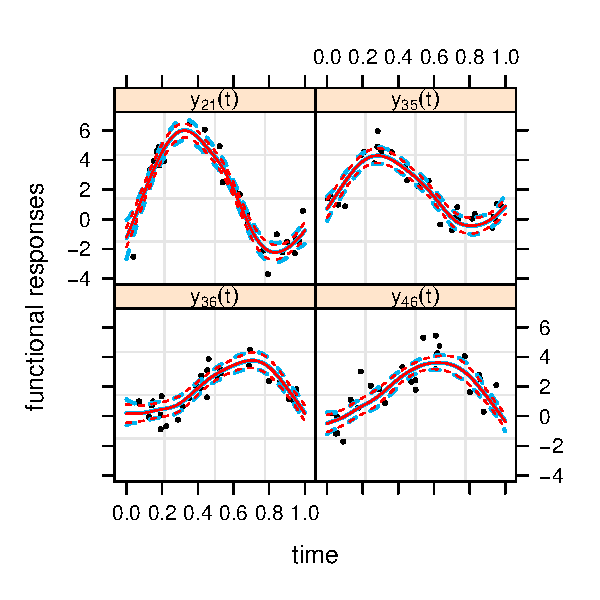
\includegraphics[width=2.3in]{images/fpca_fits.pdf}
	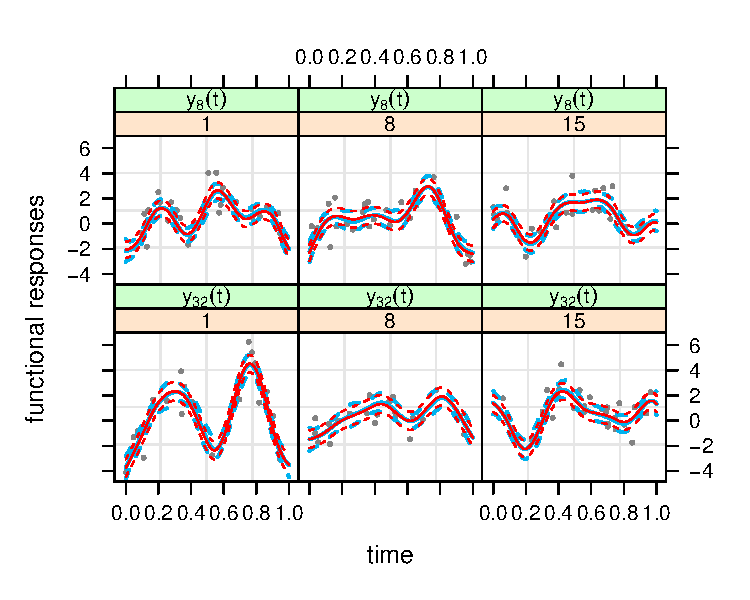
\includegraphics[width=2.9in]{images/mlfpca_fits.pdf}
\caption{
	\emph{Left panel}: One set of predictions from a simulation of the Bayesian FPCA model
	in \eqref{bayes_fpca_mod}. The simulated data are shown in black, while the VMP-based
	variational Bayes posterior estimates are presented in red and the corresponding MCMC estimates
	are shown in blue. In each panel, the solid lines represent the pointwise posterior mean, while the dashed lines
	represents the 95\% pointwise credible sets for the mean.
	\emph{Right panel}: An analogous set of plots for the Baysian MlFPCA model in
	\eqref{bayes_mlfpca_mod}. The subscripts for each $y$ in the green panels represent the first level
	index $i$, while the numbers in the orange panels represent the second level index $j$.
}
\label{fig:fpca_pred}
\end{figure}

We illustrate the use of Algorithms \ref{alg:fpca_gauss_lik_frag}, \ref{alg:mean_fpc_gauss_pen_frag} and
\ref{alg:mlfpca_gauss_lik_frag}
through a series of simulations of models \eqref{bayes_fpca_mod} and \eqref{bayes_mlfpca_mod}.
Pseudocode for the VMP algorithm for the standard FPCA model \eqref{bayes_fpca_mod} and
the MlFPCA model \eqref{bayes_mlfpca_mod} are provided in Algorithms \ref{alg:vmp_alg}
and \ref{alg:vmp_ml_alg} of Appendix \ref{app:vmp_algs}.
In addition, we have included the results from MCMC
treatments of both models for comparison with
the VMP-based variational Bayesian inference.
MCMC simulations were conducted through \textsf{Rstan}, the \textsf{R} \citep{r20} interface to the probabilistic
programming language \textsf{Stan} \citep{rstan20}.

%\begin{figure}
%	\centering
%	\begin{subfigure}[t]{0.39\textwidth}
%		\centering
%		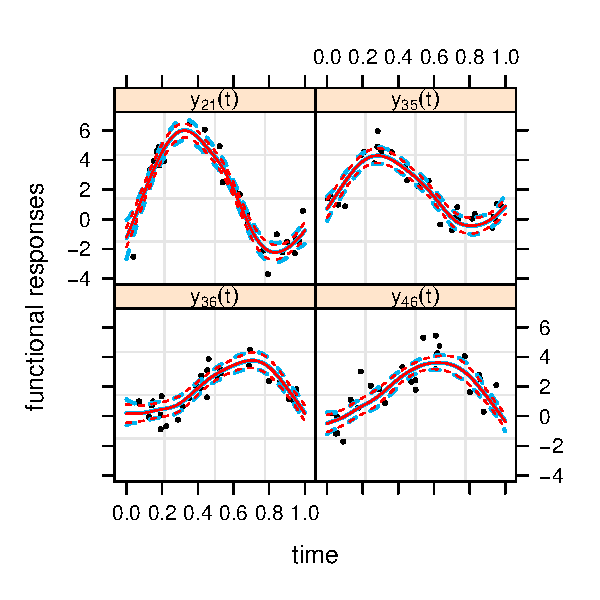
\includegraphics[height=2.5in, width = 2.2in]{images/fpca_fits.pdf}
%	\caption{}
%	\label{subfig:fpca_fits}
%	\end{subfigure}
%	%
%	\begin{subfigure}[t]{0.59\textwidth}
%		\centering
%		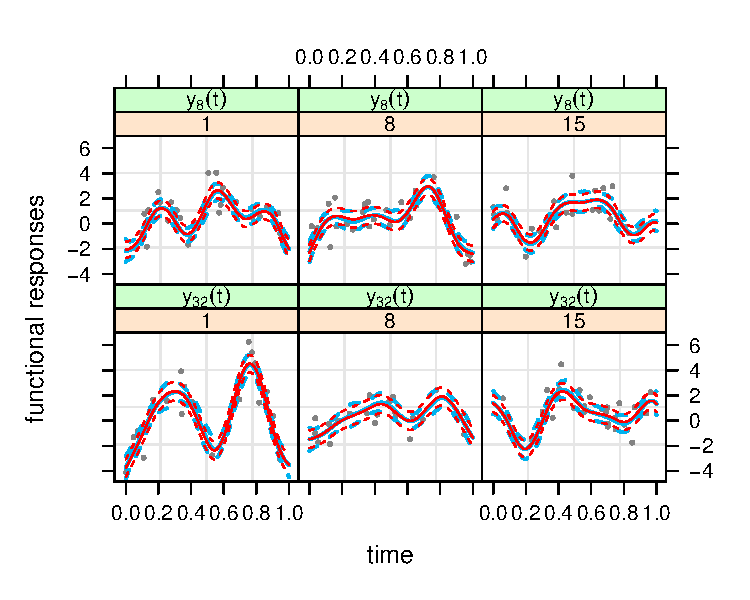
\includegraphics[height=2.5in, width = 3.3in]{images/mlfpca_fits.pdf}
%	\caption{}
%	\label{subfig:mlfpca_fits}
%	\end{subfigure}
	%
%\caption{
%	One set of predictions from simulations of \subref{subfig:fpca_fits} the Bayesian FPCA model
%	in \eqref{bayes_fpca_mod} and \subref{subfig:mlfpca_fits} the Bayesian MlFPCA model in
%	\eqref{bayes_mlfpca_mod}.
%	The simulated data are shown in black, while the VMP-based
%	variational Bayes posterior estimates are presented in red and the corresponding MCMC estimates
%	are shown in blue. In each panel, the solid lines represent
%	the posterior mean, while the dashed lines represents the 95\% pointwise credible sets for the mean.
%}
%\label{fig:gauss_resp_sim}
%\end{figure}

%%%%%%%%%%%%%% Accuracy Assessment

\subsection{Accuracy Assessment}
\label{sec:acc_ass}

%\begin{figure}
%	\centering
%	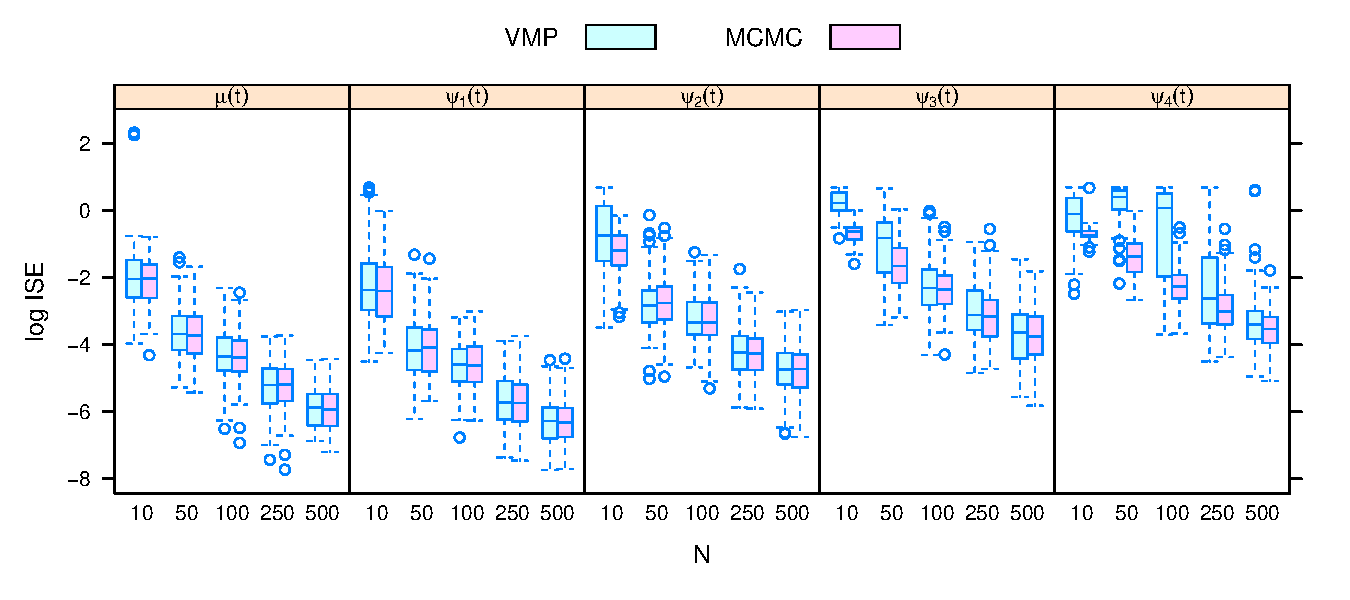
\includegraphics[height=2in]{images/box_plot_fpca_sims.pdf}
%\caption{
%	The results from a simulation study of the Bayesian FPCA model in
%	\eqref{bayes_fpca_mod}.
%	The box plots in each panel are a summary of the logarithm of the
%	integrated squared error values in \eqref{ise}
%	for 100 simulations of each of the settings $n \in \{ 10, 50, 100, 250, 500 \}$. We have also included the
%	corresponding accuracy results for the MCMC algorithm applied to \eqref{bayes_fpca_mod}.
%}
%\label{fig:fpca_sims}
%\end{figure}

For a simple illustration of the fits for the FPCA model \eqref{bayes_fpca_mod},
we simulated 50 response curves with the number
of observations $T_i$ for the $i$th curve sampled uniformly over $\{ 20, 21, \dots, 30 \}$. Furthermore, the time
observations for the $i$th curve $\{ t_{i1}, \dots, t_{i T_i} \}$ were sampled uniformly over the interval $(0, 1)$,
while the residual variance $\sigsqeps$ was set to 1. The mean function was $\mu (t) = 3 \sin (\pi t) - 1.5$
and the eigenfunctions were $\psi_1 (t) = \sqrt{2} \sin (2 \pi t)$, $\psi_2 (t) = \sqrt{2} \cos (2 \pi t)$,
$\psi_3 (t) = \sqrt{2} \sin (4 \pi t)$ and $\psi_4 (t) = \sqrt{2} \cos (4 \pi t)$.
Each principal component score was simulated according to
$\zeta_{il} \indsim \normal (0, 1/l^2)$, $i = 1, \dots, 50$, $l = 1, \dots, 4$.
Nonparameteric regression with O'Sullivan penalized splines for the nonlinear curves was performed
with $K = 10$. A similar simulation was conducted for model \eqref{bayes_mlfpca_mod} with the additional
parameters $m_i$ sampled uniformly over $\{ 10, 11, \dots, 15 \}$,
$\psi^{(1)}_1 (t) = \sqrt{2} \sin (2 \pi t)$, $\psi^{(1)}_2 (t) = \sqrt{2} \cos (2 \pi t)$, $\psi^{(1)}_3 (t) = \sqrt{2} \sin (4 \pi t)$,
$\psi^{(2)}_1 (t) = \sqrt{2} \cos (4 \pi t)$, $\psi^{(2)}_2 (t) = \sqrt{2} \sin (6 \pi t)$, $\psi^{(2)}_3 (t) = \sqrt{2} \cos (6 \pi t)$
and $\zeta^{(r)}_{il} \indsim \allowbreak \normal (0, 1/l^2)$, $i = 1, \dots, 50$, $l = 1, 2, 3$, $r = 1, 2$. The results for the FPCA
model are presented in the left panel of Figure \ref{fig:fpca_pred} where a random sample of
four of the functional responses were selected for visual clarity. Likewise, the results for the MlFPCA model
are presented in the right panel Figure \ref{fig:fpca_pred}, where two subjects were randomly selected
with three evenly temporal spaced functional reponses.
In the simulations of both models, we see strong agreement between
the VMP and MCMC predictions, as well as good predictions on the response data.
In particular, the post-VMP procedures that are outlined in Section \ref{sec:post_vmp_steps} neatly
complement the VMP algorithms.

We then incorporated five settings for the number of response curves: $n \in \{ 10, 50, \allowbreak 100, 250, 500 \}$. For each of these
settings, we conducted 100 simulations of model \eqref{bayes_fpca_mod} with the aim of analysing the error of
the posterior estimates of the mean function and the functional principal
component eigenfunctions. The error of each simulation was determined via the
integrated squared error:

\begin{equation}
	\text{ISE} (f, \fhat) = \int_0^1 \left| f (x) - \fhat(x) \right|^2 dx,
\label{ise}
\end{equation}

\noindent where, in our simulations, $f (\cdot)$ represents the true function that generated the data, while $\fhat (\cdot)$
represents the Bayesian posterior estimate. In addition, we conducted a similar series of
simulations for model \eqref{bayes_mlfpca_mod}. For comparison, we also present the analogous accuracy scores for
the MCMC algorithms.

\begin{figure}
	\centering
	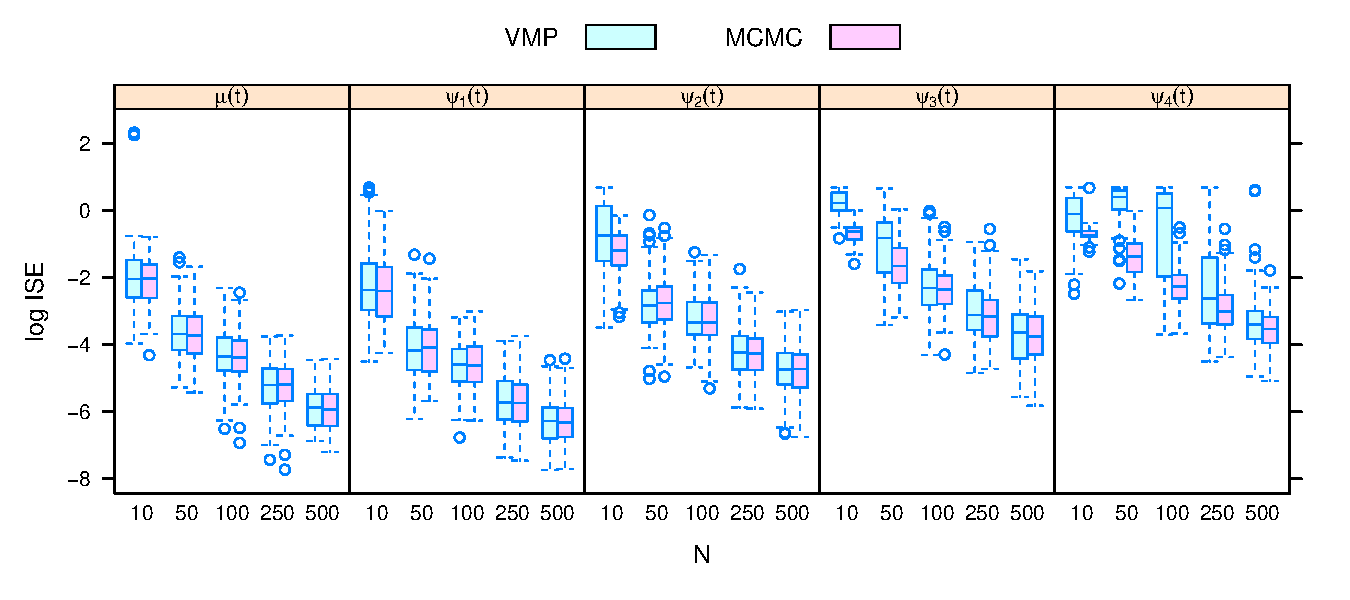
\includegraphics[width = \textwidth]{images/box_plot_fpca_sims.pdf}
	%
	\\
	%
	\centering
	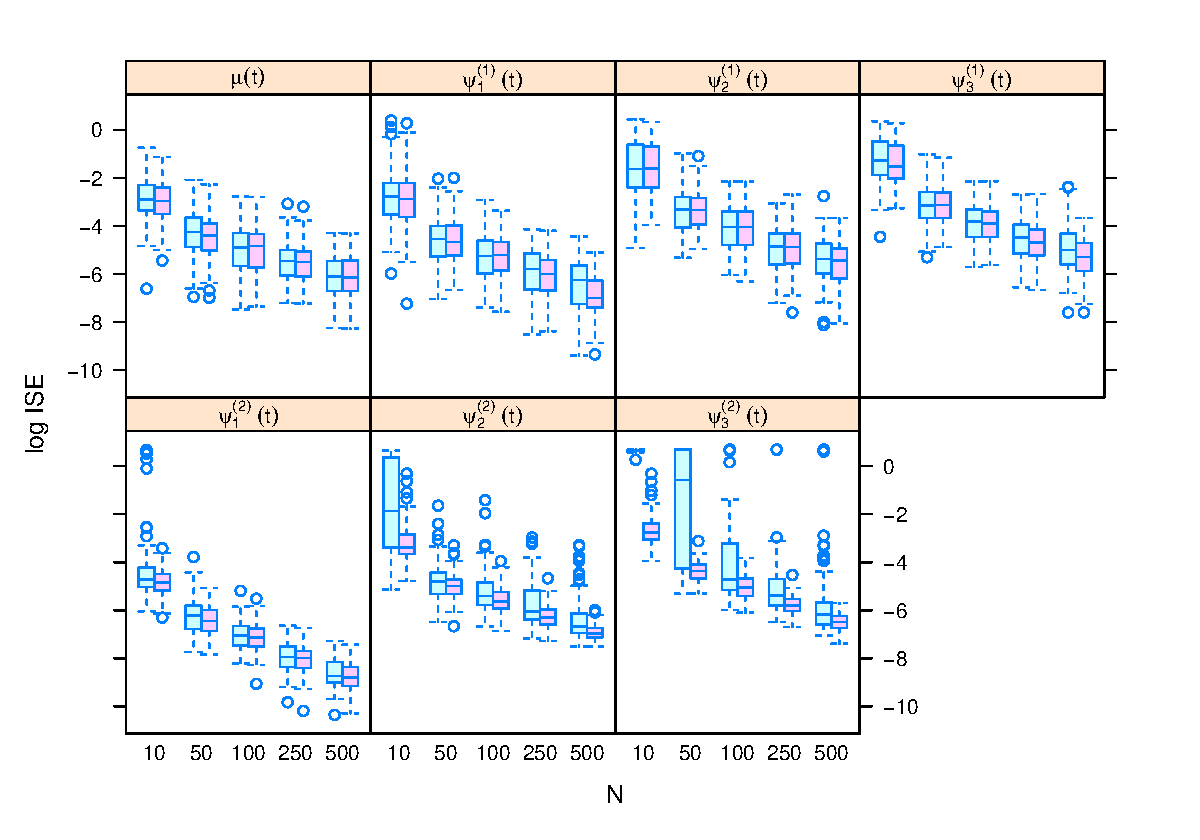
\includegraphics[height=3.6in]{images/box_plot_mlfpca_sims.pdf}
	%
\caption{
	\emph{Top panel}: The results from a simulation study of the Bayesian FPCA model in
	\eqref{bayes_fpca_mod}. \emph{Bottom panel}: Analogous results for the Bayesian MlFPCA model in
	\eqref{bayes_mlfpca_mod}.
	The box plots in each panel are a summary of the logarithm of the
	integrated squared error values in \eqref{ise}
	for 100 simulations of each of the settings $n \in \{ 10, 50, 100, 250, 500 \}$. We have also included the
	corresponding accuracy results for the MCMC algorithms.
}
\label{fig:fpca_sims}
\end{figure}

%\begin{figure}
%	\centering
%	\begin{subfigure}[t]{\textwidth}
%		\centering
%		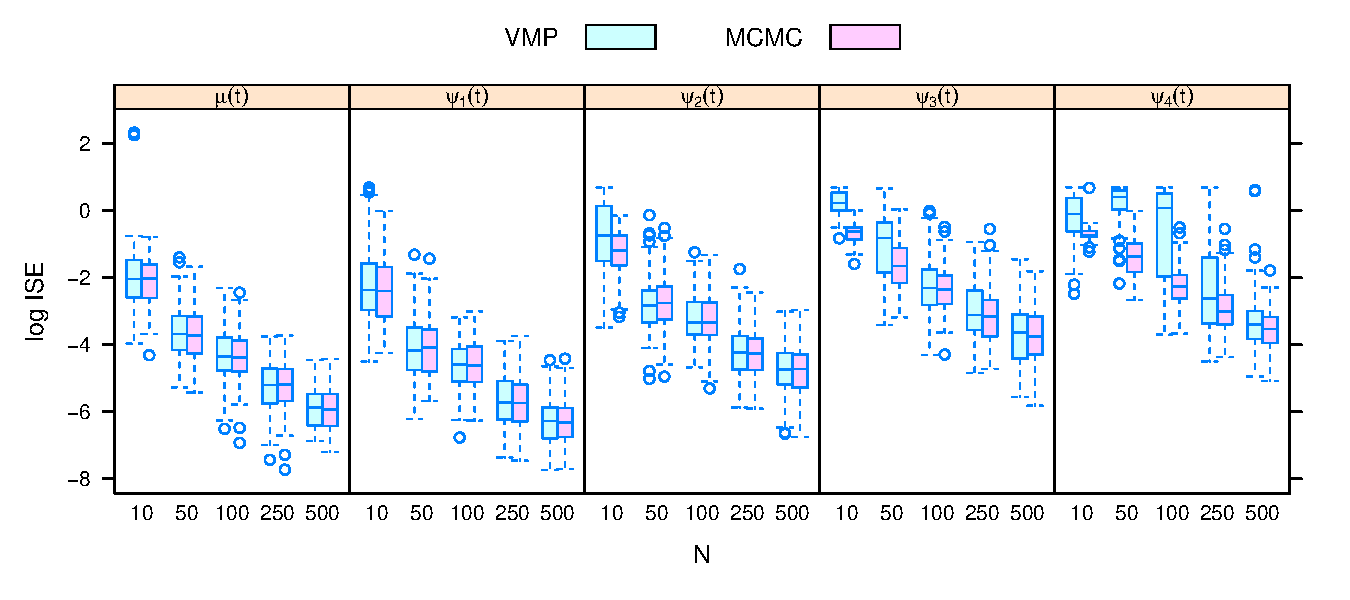
\includegraphics[height=1.5in]{images/box_plot_fpca_sims.pdf}
%	\caption{}
%	\label{subfig:fpca_sims}
%	\end{subfigure}
%	%
%	\begin{subfigure}[t]{\textwidth}
%		\centering
%		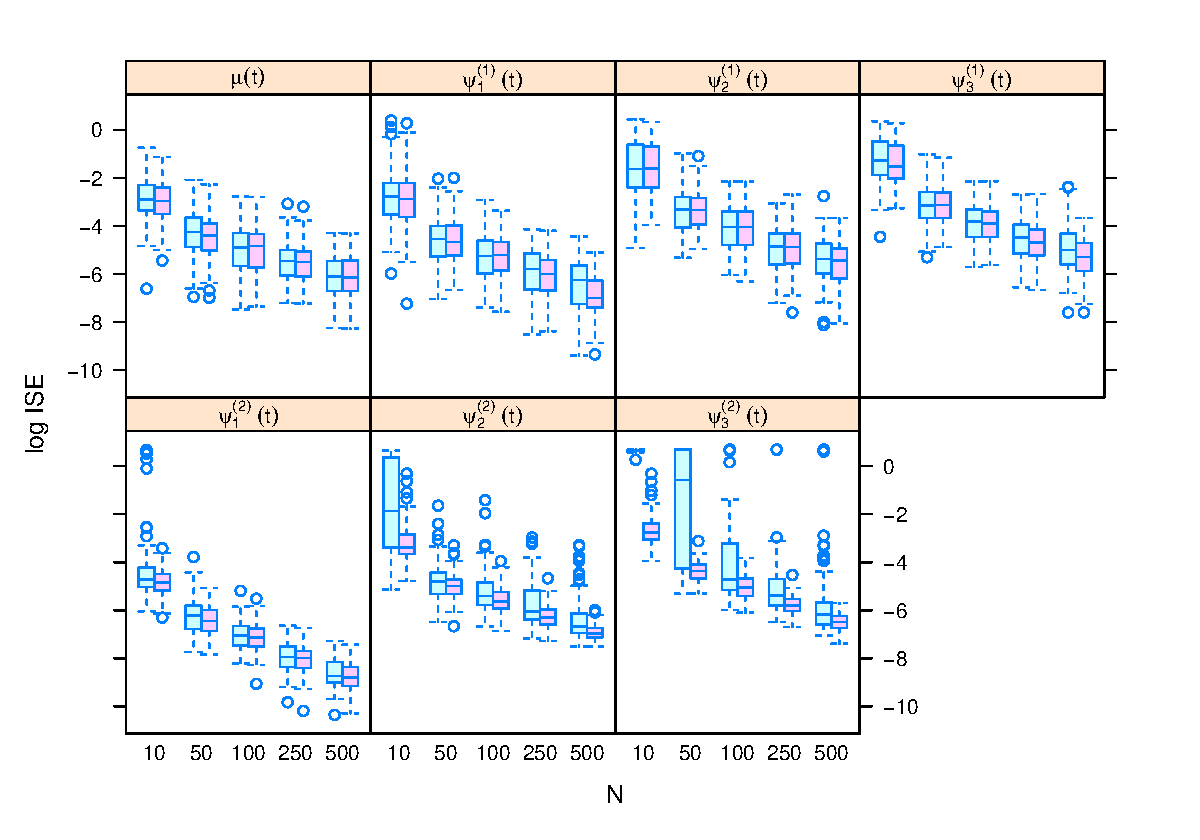
\includegraphics[height=1.5in]{images/box_plot_mlfpca_sims.pdf}
%	\caption{}
%	\label{subfig:mlfpca_sims}
%	\end{subfigure}
%	%
%\caption{
%	The results from a simulation study of \subref{subfig:fpca_sims} the Bayesian FPCA model in
%	\eqref{bayes_fpca_mod} and \subref{subfig:mlfpca_sims} the Bayesian MlFPCA model in
%	\eqref{bayes_mlfpca_mod}.
%	The box plots in each panel are a summary of the logarithm of the
%	integrated squared error values in \eqref{ise}
%	for 100 simulations of each of the settings $n \in \{ 10, 50, 100 \}$. We have also included the
%	corresponding accuracy results for the MCMC algorithms.
%}
%\label{fig:gauss_resp_sim_st}
%\end{figure}

The box plots for the logarithm of the integrated squared error values for the FPCA model
in Figure \ref{fig:fpca_sims} reflect the overall excellent results of the VMP algorithms.
For lower values of $n$, the log ISE for $\psi_4 (t)$ tends to be greater for the VMP simulations
than the MCMC simulations. This fall off in accuracy for the VMP simulations is a result
of the weak contribution of this eigenfunction to the variability of the dataset, where it accounts for
approximately 4.4\% of the total variability. Similar results are also observed for the MlFPCA simulations.

%\begin{figure}
%	\centering
%	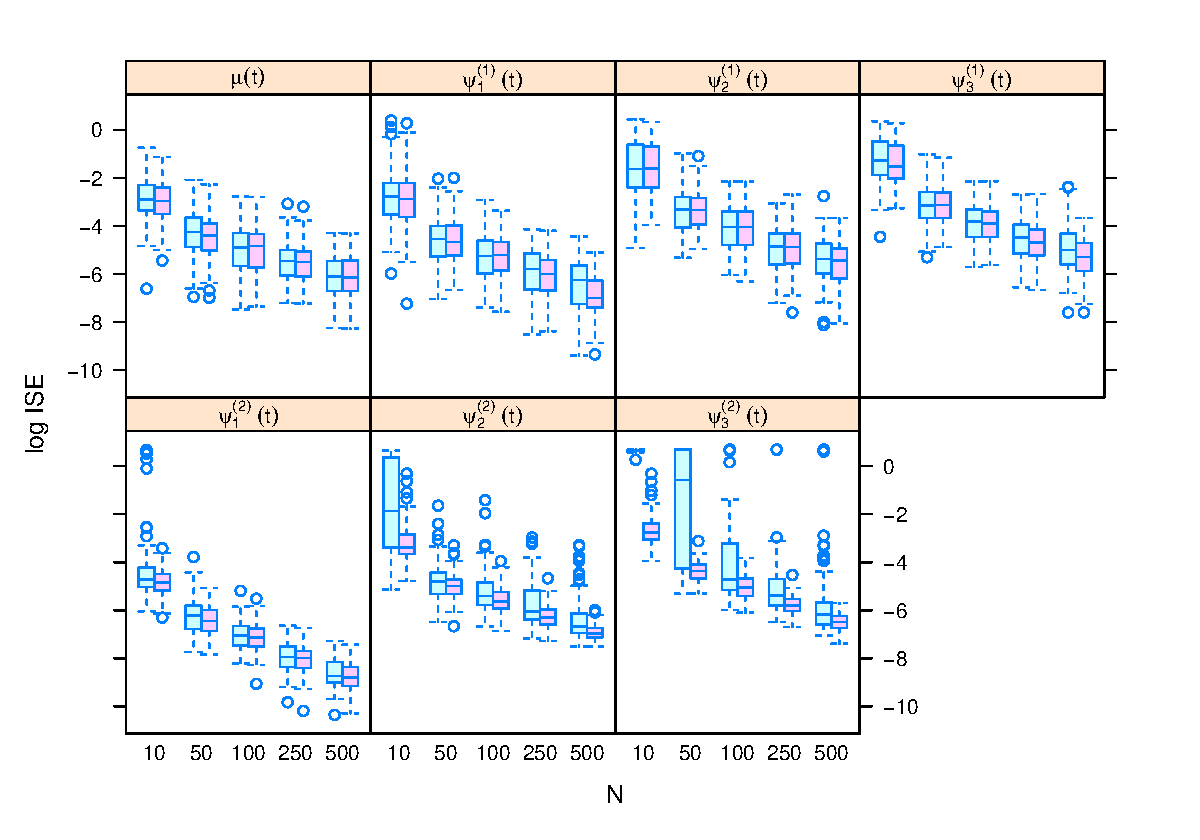
\includegraphics[height=2in]{images/box_plot_mlfpca_sims.pdf}
%\caption{
%	An analogous set of accuracy results to Figure \ref{fig:fpca_sims} for a simulation study of the
%	the Bayesian MlFPCA model in \eqref{bayes_mlfpca_mod}.
%}
%\label{fig:mlfpca_sims}
%\end{figure}

To assess the accuracy in the estimation of the scores, we used the root mean squared error (RMSE).
The results are listed in Table \ref{tab:fpca_scores} for the FPCA and the MlFPCA models via VMP and MCMC.
The RMSE values for the posterior estimates of the scores in the VMP simulations match well with the MCMC
simulations.

\begin{table}
\begin{center}
\begin{tcolorbox}[size=tight,on line,left=0mm,right=0mm,width=1\textwidth,bottom=0mm,top=1mm,arc=0mm,outer arc=0pt, box align=center,boxrule=1.5pt]
\captionsetup{width=0.9\textwidth}
\captionof{table}{
	Median (median absolute deviation) RMSE for the scores.
}
\begin{tabularx}{\textwidth}{>{\hsize=.2\hsize}X | >{\hsize=.4\hsize}X | >{\hsize=.4\hsize}X}
	\hline \hline
	\multicolumn{3}{c}{FPCA model} \\
	\hline
	\rowcolor[gray]{.8}
	\centering $n$ & \centering VMP & \centering\arraybackslash MCMC \\
	\rowcolor{white!50}
	\centering 10 & \centering 0.66 (0.06) & \centering\arraybackslash 0.62 (0.03) \\
	\rowcolor{white!50}
	\centering 50 & \centering 0.65 (0.07) & \centering\arraybackslash 0.62 (0.04) \\
	\rowcolor{white!50}
	\centering 100 & \centering 0.66 (0.07) & \centering\arraybackslash 0.62 (0.04) \\
	\rowcolor{white!50}
	\centering 250 & \centering 0.65 (0.06) & \centering\arraybackslash 0.62 (0.04) \\
	\rowcolor{white!50}
	\centering 500 & \centering 0.65 (0.07) & \centering\arraybackslash 0.62 (0.04) \\
	\hline \hline
\end{tabularx}
\begin{tabularx}{\textwidth}{>{\hsize=.2\hsize}X | >{\hsize=.2\hsize}X | >{\hsize=.2\hsize}X | >{\hsize=.2\hsize}X | >{\hsize=.2\hsize}X}
	\multicolumn{5}{c}{MlFPCA model} \\
	\hline
	\rowcolor[gray]{.8}
	\centering $n$ & \centering VMP ($\bzetaL{1}{}$) & \centering MCMC ($\bzetaL{1}{}$) & \centering VMP ($\bzetaL{2}{}$) & \centering\arraybackslash MCMC ($\bzetaL{2}{}$) \\
	\rowcolor{white!50}
	\centering 10 & \centering 0.45 (0.10) & \centering 0.40 (0.09) & \centering 0.64 (0.10) & \centering\arraybackslash 0.56 (0.08) \\
	\rowcolor{white!50}
	\centering 50 & \centering 0.43 (0.09) & \centering 0.39 (0.08) & \centering 0.62 (0.09) & \centering\arraybackslash 0.56 (0.11) \\
	\rowcolor{white!50}
	\centering 100 & \centering 0.45 (0.10) & \centering 0.41 (0.10) & \centering 0.63 (0.11) & \centering\arraybackslash 0.58 (0.09) \\
	\rowcolor{white!50}
	\centering 250 & \centering 0.42 (0.08) & \centering 0.40 (0.07) & \centering 0.62 (0.09) & \centering\arraybackslash 0.56 (0.09) \\
	\rowcolor{white!50}
	\centering 500 & \centering 0.44 (0.08) & \centering 0.40 (0.08) & \centering 0.63 (0.10) & \centering\arraybackslash 0.57 (0.07) \\
	\hline
\end{tabularx}
\label{tab:fpca_scores}
\end{tcolorbox}
\end{center}
\end{table}

%%%%%%%%%%%%%% Computational Speed Comparisons

\subsection{Computational Speed Comparisons}
\label{sec:speed_comp}

In the previous section, we saw that the mean field product restriction in \eqref{fpca_mf_restrn} does not
compromise the accuracy of variational Bayesian inference for FPCA and similarly for MlFPCA. Another
major advantage offered by variational Bayesian inference via VMP is fast approximate inference in 
comparison to MCMC simulations. Several published articles have addressed the computational speed gains
from using variational Bayesian inference. \citet{faes11} presented speed gains for parametric and nonparametric
regression with missing data, \citet{luts15} presented timing comparisons for semiparametric regression
models with count responses, and
\citet{lee16} and \citet{nolanmw20} established speed gains for multilevel data models
with streamlined matrix algebraic results.
In all cases, the variational Bayesian inference algorithms had strong accuracy in
comparison to MCMC simulations and were far superior in computational speed.

In Table \ref{tab:fpca_speed}, we present a similar set of results for the computational speed of VMP and MCMC
for models \eqref{bayes_fpca_mod}
and \eqref{bayes_mlfpca_mod}. The simulations were identical to those that were used to generate the
results in Figure \ref{fig:fpca_sims}. In Table \ref{tab:fpca_speed},
we present the median elapsed computing time (in seconds),
with the median absolute deviation in brackets. For the FPCA results,
notice that most of the VMP simulations are completed within one minute, whereas the elapsed computing times
for the MCMC simulations can exceed one hour for $n = 500$.
The most impressive results are in the fourth column, where the median VMP simulations are shown to
be roughly 25--100 times faster, depending on the values of $n$. A similar set of results are observed
for the Bayesian MlFPCA model.

\begin{table}
\begin{center}
\begin{tcolorbox}[size=tight,on line,left=0mm,right=0mm,width=1\textwidth,bottom=0mm,top=1mm,arc=0mm,outer arc=0pt, box align=center,boxrule=1.5pt]
\captionsetup{width=0.9\textwidth}
\captionof{table}{
	Median (median absolute deviation) elapsed computing time for conducting Bayesian FPCA
	and Bayesian MlFPCA
	in seconds for VMP and MCMC  with
	$n \in (10, 50, 100, 250, 500)$. The fourth column presents the ratio of the median elapsed time for MCMC
	to the median elapsed time for VMP.
	The fifth column shows the median (median absolute deviation) number of VMP iterations prior to convergence.
}
\begin{tabularx}{\textwidth}{>{\hsize=.05\hsize}X | >{\hsize=.2\hsize}X | >{\hsize=.27\hsize}X | >{\hsize=.17\hsize}X | >{\hsize=.21\hsize}X}
	\hline \hline
	\multicolumn{5}{c|}{FPCA model} \\
	\hline
	\rowcolor[gray]{.8}
	\centering $n$ & \centering VMP & \centering MCMC & \centering MCMC/VMP & \centering\arraybackslash VMP Iterations \\
	\rowcolor{white!50}
	\centering 10 & \centering 4.9 (2.0) & \centering 122.6 (17.7) & \centering 24.9 & \centering\arraybackslash 130 (64) \\
	\rowcolor{white!50}
	\centering 50 & \centering 8.1 (3.1) & \centering 310.0 (30.9) & \centering 38.2 & \centering\arraybackslash 51 (22) \\
	\rowcolor{white!50}
	\centering 100 & \centering 15.6 (4.7) & \centering 609.3 (34.8) & \centering 39.2 & \centering\arraybackslash 58 (18) \\
	\rowcolor{white!50}
	\centering 250 & \centering 32.0 (7.4) & \centering 2564.7 (570.5) & \centering 80.0 & \centering\arraybackslash 46 (9) \\
	\rowcolor{white!50}
	\centering 500 & \centering 59.3 (15.9) & \centering 5841.8 (889.6) & \centering 98.5 & \centering\arraybackslash 41 (9) \\
	\hline \hline
	\multicolumn{5}{c|}{MlFPCA model} \\
	\hline
	\rowcolor[gray]{.8}
	\centering $n$ & \centering VMP & \centering MCMC & \centering MCMC/VMP & \centering\arraybackslash VMP Iterations \\
	\rowcolor{white!50}
	\centering 10 & \centering 28.3 (16.9) & \centering 1771.6 (247.2) & \centering 62.7 & \centering\arraybackslash 104 (79) \\
	\rowcolor{white!50}
	\centering 50 & \centering 211.8 (83.1) & \centering 13789.0 (1194.0) & \centering 65.1 & \centering\arraybackslash 120 (91) \\
	\rowcolor{white!50}
	\centering 100 & \centering 453.9 (205.8) & \centering 30938.9 (5250.9) & \centering 68.2 & \centering\arraybackslash 223 (111) \\
	\rowcolor{white!50}
	\centering 250 & \centering 975.0 (519.1) & \centering 69845.4 (11572.5) & \centering 71.6 & \centering\arraybackslash 196 (116) \\
	\rowcolor{white!50}
	\centering 500 & \centering 2906.7 (1311.5) & \centering 216260.0 (70246.9) & \centering 74.4 & \centering\arraybackslash 211 (100) \\
	\hline
\end{tabularx}
\label{tab:fpca_speed}
\end{tcolorbox}
\end{center}
\end{table}

The speed of the VMP algorithm is dependent on the convergence of the lower bound on the marginal
log-likelihood (see Appendix \ref{app:convergence}). These results are summarized in column 5 of
Table \ref{tab:fpca_speed}, where the median number of iterations (with median absolute deviation in
brackets) are presented. Most of the FPCA simulations converged within 150 iterations. Similarly, most
of the MlFPCA simulations converged within 250 iterations.

%\begin{figure}
%	\centering
%	\begin{subfigure}[t]{0.49\textwidth}
%		\centering
%		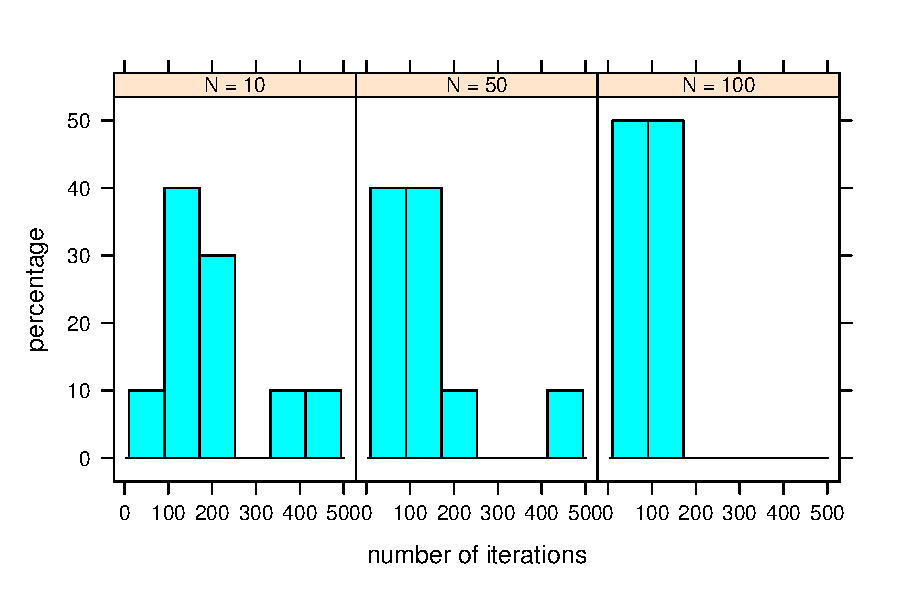
\includegraphics[width=2.6in]{images/hist_fpca_iters.pdf}
%	\caption{}
%	\label{subfig:fpca_convergence}
%	\end{subfigure}
%	%
%	\begin{subfigure}[t]{0.49\textwidth}
%		\centering
%		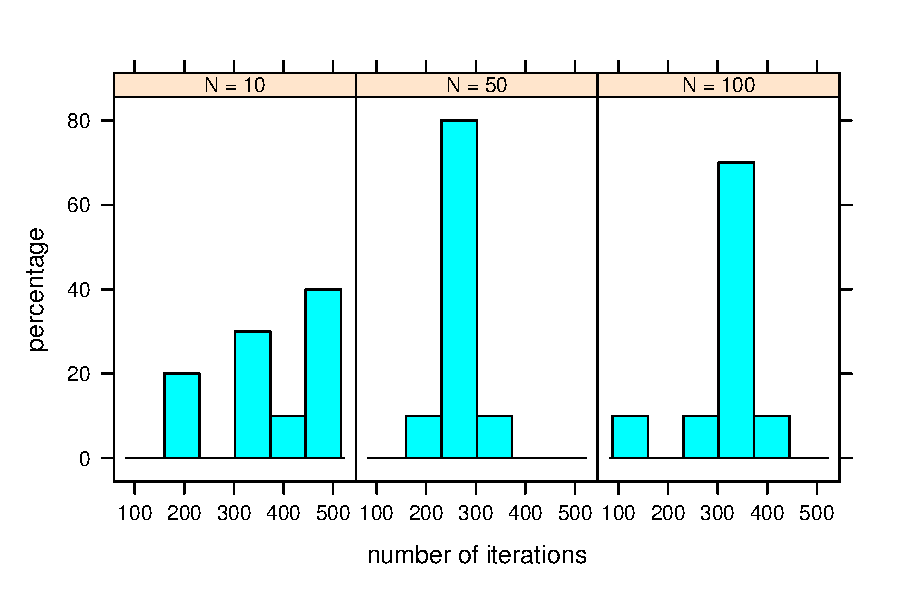
\includegraphics[width=2.6in]{images/hist_mlfpca_iters.pdf}
%	\caption{}
%	\label{subfig:mlfpca_convergence}
%	\end{subfigure}
%	%
%\caption{
%	Convergence of the algorithms for
%	\subref{subfig:fpca_convergence} FPCA and \subref{subfig:mlfpca_convergence} MlFPCA
%	via VMP.
%}
%\label{fig:convergence}
%\end{figure}

%%%%%%%%%%%%%% Determining the Number of Non-zero Eigenvalues

%\subsection{The Number of Non-zero Eigenvalues}
%\label{sec:non_zero_eigs}

%The number of non-zero eigenvalues $L$ is an input into the Bayesian FPCA model \eqref{bayes_fpca_mod}.
%Likewise, $L_1$ and $L_2$ are also inputs into the Bayesian MlFPCA model \eqref{bayes_mlfpca_mod}. Here,
%we provide a simple means of determining the number of non-zero eigenvalues. We applied VMP and MCMC to
%model \eqref{bayes_fpca_mod} with similar simulation parameters to Section \ref{sec:acc_ass}, but setting
%$n = 100$ and including the additional scenario of $L \in \{ 2, 4, 6 \}$. The results, summarized in
%Table \ref{tab:fpca_exp_var} as the cumulative proportion of the explained variability for each eigenfunction,
%show good agreement between both the VMP and MCMC algorithms. Noting that the true number of non-zero
%eigenvalues is 4, we propose that the best way to estimate the number of non-zero eigenvalues is to progressively
%increase $L$ until the cumulative proportion of explained variability estimates has converged. From Table
%\ref{tab:fpca_exp_var}, we see that this converges by $L = 4$ for the simulated data.

%\begin{table}
%\begin{center}
%\begin{tcolorbox}[size=tight,on line,left=0mm,right=0mm,width=1\textwidth,bottom=0mm,top=1mm,arc=0mm,outer arc=0pt, box align=center,boxrule=1.5pt]
%\captionsetup{width=0.9\textwidth}
%\captionof{table}{
%	Median cumulative proportion of the explained variability for
%	the first six eigenfunctions.
%}
%\begin{tabularx}{\textwidth}{
%	>{\hsize=.1\hsize}X |
%	>{\hsize=.15\hsize}X | >{\hsize=.15\hsize}X | >{\hsize=.15\hsize}X |
%	>{\hsize=.15\hsize}X | >{\hsize=.15\hsize}X | >{\hsize=.15\hsize}X
%}
%	\hline \hline
%	\multicolumn{7}{c}{VMP} \\
%	\hline
%	\rowcolor[gray]{.8}
%	\centering $L$ & \centering $\psi_1$ & \centering $\psi_2$ & \centering $\psi_3$
%		& \centering $\psi_4$ & \centering $\psi_5$ & \centering\arraybackslash $\psi_6$ \\
%	\rowcolor{white!50}
%	\centering 2 & \centering 0.82 & \centering\arraybackslash 1 & \centering\arraybackslash 1
%		 & \centering\arraybackslash 1 & \centering\arraybackslash 1 & \centering\arraybackslash 1 \\
%	\rowcolor{white!50}
%	\centering 4 & \centering 0.78 & \centering\arraybackslash 0.94 & \centering\arraybackslash 0.99
%		 & \centering\arraybackslash 1 & \centering\arraybackslash 1 & \centering\arraybackslash 1 \\
%	\rowcolor{white!50}
%	\centering 6 & \centering 0.77 & \centering\arraybackslash 0.92 & \centering\arraybackslash 0.98
%		 & \centering\arraybackslash 1 & \centering\arraybackslash 1 & \centering\arraybackslash 1 \\
%	\hline \hline
%	\multicolumn{7}{c}{MCMC} \\
%	\hline
%	\rowcolor[gray]{.8}
%	\centering $L$ & \centering $\psi_1$ & \centering $\psi_2$ & \centering $\psi_3$
%		& \centering $\psi_4$ & \centering $\psi_5$ & \centering\arraybackslash $\psi_6$ \\
%	\rowcolor{white!50}
%	\centering 2 & \centering 0.82 & \centering\arraybackslash 1 & \centering\arraybackslash 1
%		 & \centering\arraybackslash 1 & \centering\arraybackslash 1 & \centering\arraybackslash 1 \\
%	\rowcolor{white!50}
%	\centering 4 & \centering 0.76 & \centering\arraybackslash 0.92 & \centering\arraybackslash 0.98
%		 & \cenxtering\arraybackslash 1 & \centering\arraybackslash 1 & \centering\arraybackslash 1 \\
%	\rowcolor{white!50}
%	\centering 6 & \centering 0.76 & \centering\arraybackslash 0.92 & \centering\arraybackslash 0.98
%		 & \centering\arraybackslash 1 & \centering\arraybackslash 1 & \centering\arraybackslash 1 \\
%	\hline
%\end{tabularx}
%\label{tab:fpca_exp_var}
%\end{tcolorbox}
%\end{center}
%\end{table}

%%%%%%%%%%%  APPLICATION:  UNITED STATES  TEMPERATURE  DATA  %%%%%%%%%%%

\section{Application: United States Temperature Data}
\label{sec:us_weather_data}

We now provide an illustration of our methodology with an application to temperature data collected from
various United
States weather stations, which is available from the \textsf{rnoaa} package \citep{rnoaa21} in \textsf{R}.
The \textsf{rnoaa}
package is an interface to the National Oceanic and Atmospheric Administration's climate data.
The function \textsf{ghcnd\_stations()} provides access to all available global historical climatology
network daily weather data for each weather site from 1960 to 1994. The information includes the longitude
and latitude for each site, and this was used to determine site's US state.
Our analysis focused on maximum daily temperature over the 25 years of available data.
From this package, we randomly selected a single weather station from each state and collected the
weather station's daily maximum temperature recordings from 1960 to 1994.
Additionally, we partition each weather station's dataset by year.
The resulting dataset is
a multilevel functional dataset, with the state (represented by a single weather station) as the first level
and the year as the second level.

In the context of experimental design, the US temperature data
has a crossed random effects structure, where each combination of state and year is available. In general,
however, the years of recorded data need not be the same for each site. Consider, for example,
the Texas weather station missing all data from 1972, the Washington weather station missing all data
from 1986 and the California weather station only beginning temperature records after 1968. Then, the
crossed random effects structure would no longer hold. From this point of view, it makes sense to model
the weather station's state as a fixed effect (a level one variable) and the year of recorded data as a random
effect (a level two variable).

%\begin{figure}
%	\centering
%	\begin{subfigure}[t]{0.49\textwidth}
%		\centering
%		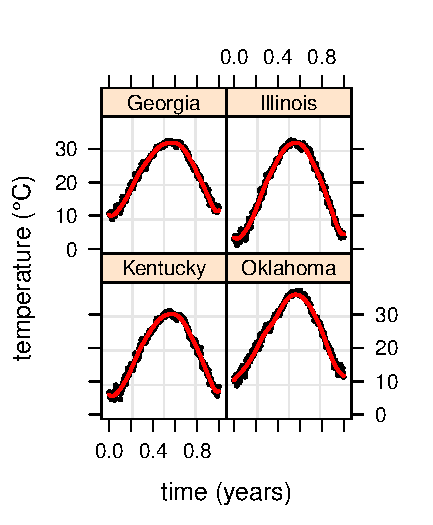
\includegraphics[width=2.6in]{images/us_fits.pdf}
%	\caption{}
%	\label{subfig:us_fits}
%	\end{subfigure}
	%
%	\begin{subfigure}[t]{0.49\textwidth}
%		\centering
%		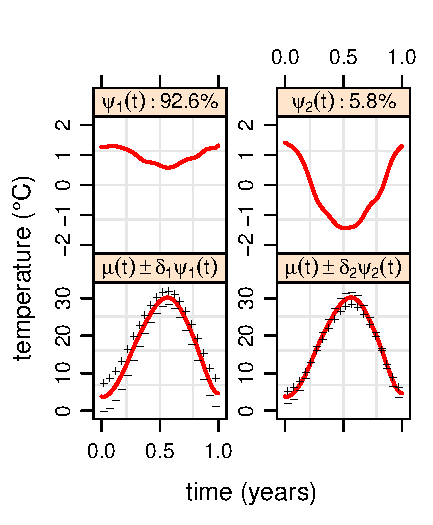
\includegraphics[width=2.6in]{images/us_bf.pdf}
%	\caption{}
%	\label{subfig:us_mean_shift}
%	\end{subfigure}
	%
%\caption{
%	Application of the VMP algorithm for FPCA to the United States temperature data. The fits in \subref{subfig:us_fits}
%	are for four randomly selected weather stations in the dataset.
%	The plots in \subref{subfig:us_mean_shift} present the pointwise posterior mean estimates of the eigenfunctions
%	(top panel) and
%	show the estimated mean function with
%	perturbations from each eigenfunction (bottom panel): $\muhat (t) \pm \delta_l \psihat_l (t)$,
%	$l = 1, 2$.
%}
%\label{fig:us_weather_data}
%\end{figure}

\begin{figure}
	\centering
	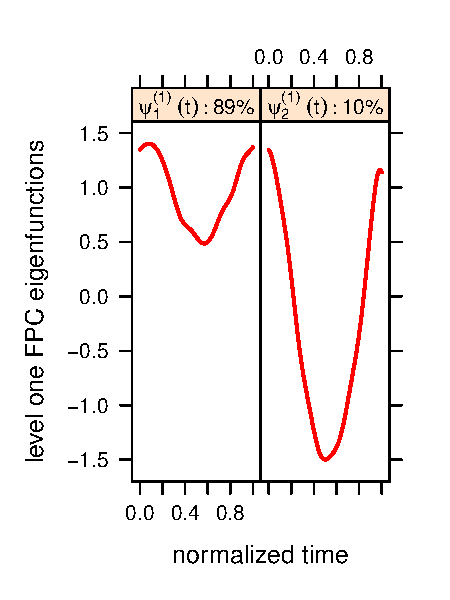
\includegraphics[width=2.3in]{images/us_ml_bf_1.pdf}
	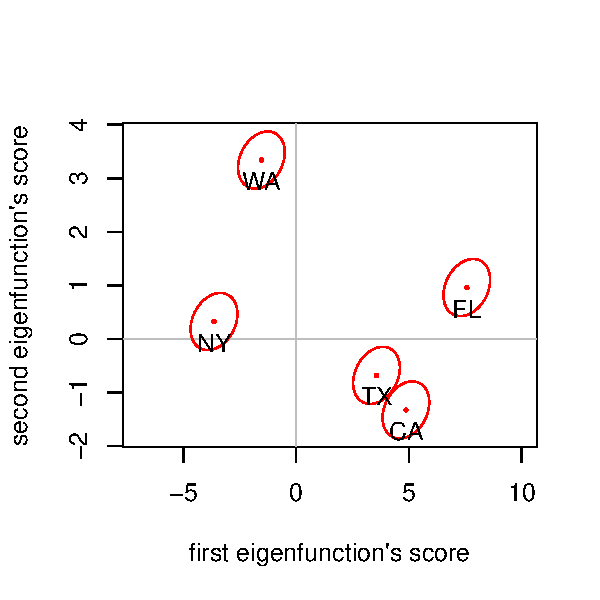
\includegraphics[width=2.9in]{images/us_scores_1.pdf} \\
	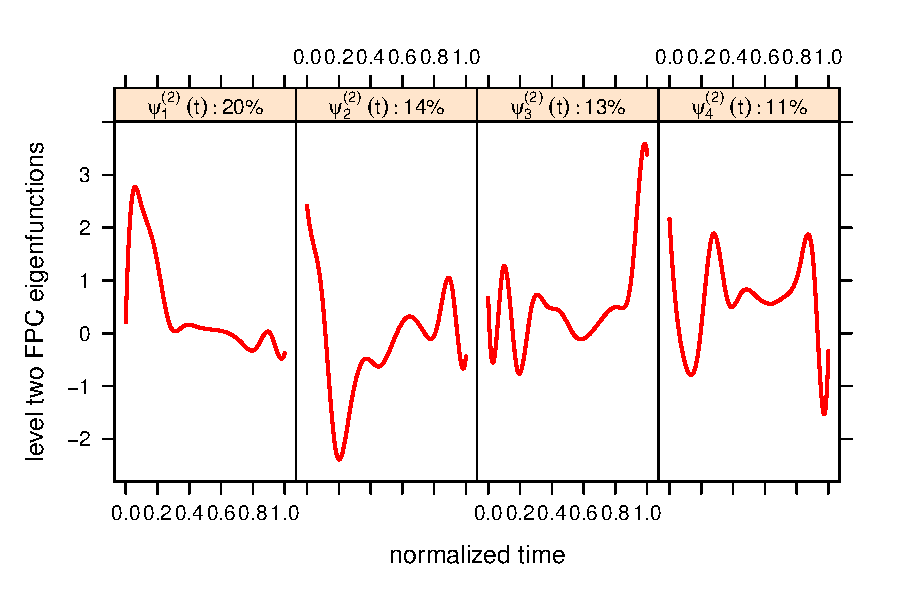
\includegraphics[width=5in]{images/us_ml_bf_2.pdf}
\caption{
	\emph{Top-left panel}: The first two eigenfunctions of the first level covariance operator. The proportion of explained
	variability for each eigenfunction is also presented.
	\emph{Top-right panel}: The corresponding scores for the weather stations in California (CA), Florida (FL), New York state (NY),
	Texas (TX) and Washington state (WA).
	\emph{Bottom panel}: The first four eigenfunctions of the second level covariance operator. The proportion of explained
	variability for each eigenfunction is also presented.
}
\label{fig:us_weather_data_L1}
\end{figure}

Chapter 8 of \citet{ramsay05} consider a similar example of Canadian temperature data from various weather
stations. The difference in our analysis, aside from collecting US data, is the multilevel structure of the
dataset. An additional consideration in the multilevel setting is the appropriate choices for $L_1$ and $L_2$,
the number of non-zero eigenvalues for the first and second level covariance operators.
In the standard Bayesian FPCA model, we progressively increase $L$ until the proportion of 
explained variability for each eigenfunction converges. For the US temperature data, we set
$L_1 = 4$ and progressively increased $L_2$ until the proportion of 
explained variability for each second level eigenfunction converged. This occurred for $L_2 = 14$.
We then conducted a similar sequence of steps by setting $L_2 = 14$ and varying $L_1$. We
found that the proportion of explained variability converged once $L_1 = 7$.

The results for the first level eigenfunctions and scores are presented in
the top-left panel of Figure \ref{fig:us_weather_data_L1}.
The first eigenfunction, which accounts for 89\% of the first level variability, is a mean shift (since it is always
positive). Its effect is stronger in the Winter months, indicating that US temperature is most variable in the
Winter. Similar analysis of the
second eigenfunction, which accounts for 11\% of the total variation, shows that it represents uniformity in the measured
temperatures. It has positive contributions in the Winter months and negative contributions in the Summer months.
As a consequence, weather stations at locations with larger discrepancies
between Winter and Summer temperatures will have a strong and negative score for this eigenfunction.
In the top-right panel of Figure \ref{fig:us_weather_data_L1}, we present the scores for the weather stations in
California (CA), Florida (FL), New York state (NY), Texas (TX) and Washington state (WA), as well as their
95\% posterior credible boundaries. Florida, California and Texas all have positive scores for the first
eigenfunction, indicating yearly maximal temperature recordings higher than the national average. New York
and Washington have negative scores for the first eigenfunction, which is indicative of their lower than average
temperatures.
The scores for the second eigenfunction indicate that the
greatest variability between Summer and Winter months can be found
in California, whereas Washington state tends to have more uniform yearly
temperature recordings.
We also present the first four second level eigenfunctions in the bottom panel of Figure \ref{fig:us_weather_data_L1}.
However, these eigenfunctions are mostly periodic and difficult to interpret.

%%%%%%%%%%%  CLOSING  REMARKS  %%%%%%%%%%%

\section{Closing Remarks}
\label{sec:closing_remarks}

We have provided a comprehensive overview of Bayesian FPCA and MlFPCA with a VMP-based mean
field variational Bayes approach. Our coverage has focused on the Gaussian likelihood specification for the observed data,
and it includes the introduction of three new fragments. In addition, a sequence of post-processing steps have
been established to satisfy the orthogonality requirements of FPCA. There are numerous extensions that cannot be included
in a single article including non-Gaussian likelihood specifications, multivariate FPCA modelling and experimentation with
other spline or wavelet families for nonparametric regression. This article provides a clear means for resolving such
methodological extensions.

%%%%%%%%%%%%%%  FUNDING  %%%%%%%%%%%%%%%

\section*{Funding}

Tui H. Nolan's research was supported by a Fulbright scholarship, an American Australian Association
scholarship and a Roberta Sykes scholarship. Jeff Goldsmith's research was supported by Award
R01NS097432 from the National Institute of Neurological Disorders and Stroke (NINDS) and by Award
R01AG062401 from the National Institute of Aging. David Ruppert's research was supported by
the National Science Foundation grant AST-1814840.

%%%%%%%%%%%%%%%%%%%%%%%%%%%%%%%%%%%%%%%%%%%%%%
%% Supplementary Material, if any, should   %%
%% be provided in {supplement} environment  %%
%% with title and short description.        %%
%%%%%%%%%%%%%%%%%%%%%%%%%%%%%%%%%%%%%%%%%%%%%%

\begin{supplement}
\stitle{Appendix \ref{app:proof_thm_orth_basis}: Proof of Theorem \ref{thm:orth_basis}}
\sdescription{A detailed proof of Theorem \ref{thm:orth_basis}.}
\end{supplement}

\begin{supplement}
\stitle{Appendix \ref{app:exp_fam_form}: Exponential Family Form}
\sdescription{An overview of the exponential family forms for the normal and inverse-$\chi^2$ density functions.}
\end{supplement}

\begin{supplement}
\stitle{Appendix \ref{app:proof_lem_response_est}: Proof of Lemma \ref{lem:response_est}}
\sdescription{A detailed proof of Lemma \ref{lem:response_est}.}
\end{supplement}

\begin{supplement}
\stitle{Appendix \ref{app:proof_prop_bi_eigenfunctions}: Proof of Proposition \ref{prop:bi_orthogonal}}
\sdescription{A detailed proof of Proposition \ref{prop:bi_orthogonal}.}
\end{supplement}

\begin{supplement}
\stitle{Appendix \ref{app:fpca_gauss_lik_frag}: Derivation of the Functional Principal Component Gaussian Likelihood Fragment}
\sdescription{A derivation of the VMP updates presented in Algorithm \ref{alg:fpca_gauss_lik_frag}.}
\end{supplement}

\begin{supplement}
\stitle{Appendix \ref{app:mean_fpc_gauss_pen_frag}: Derivation of the Functional Principal Component Gaussian Penalization Fragment}
\sdescription{A derivation of the VMP updates presented in Algorithm \ref{alg:mean_fpc_gauss_pen_frag}.}
\end{supplement}

\begin{supplement}
\stitle{Appendix \ref{app:two_lev_sparse_mat}: Two-level Sparse Matrix Background}
\sdescription{An overview of the two-level sparse matrix problems in VMP from \citet{nolanmw20}.}
\end{supplement}

\begin{supplement}
\stitle{Appendix \ref{app:mlfpca_gauss_lik_frag}: Derivation of the Multilevel Functional Principal Component Gaussian Likelihood Fragment}
\sdescription{A derivation of the VMP updates presented in Algorithm \ref{alg:mlfpca_gauss_lik_frag}.}
\end{supplement}

\begin{supplement}
\stitle{Appendix \ref{app:conv_updates}: Convergence and Algorithmic Updates}
\sdescription{A description of the convergence of the VMP algorithms and pseudocode for the Bayesian FPCA and MlFPCA models.}
\end{supplement}


\bibliographystyle{ba}
\bibliography{bibliography}

%\begin{acks}[Acknowledgments]
%And this is an acknowledgements section with a heading that was produced by the
%$\backslash$section* command. Thank you all for helping me writing this
%\LaTeX\ sample file.
%\end{acks}


\end{document}

